\documentclass[12pt,letterpaper]{report}
%
% Review cuthesis.sty for more documentation on available options
% for this package.

% Leave the below option as "masters," as it generates "thesis" on title page. 
% PhD generates "dissertation" and that word is not recognized by Carleton Library
\usepackage[masters,2committee]{cuthesis}
\usepackage{array}
\usepackage{graphicx}
\usepackage{cite}
\usepackage{subfigure}
\usepackage{amsmath}
\usepackage[indent,bf]{caption}
\usepackage{rotating}
\usepackage{setspace}
\usepackage{longtable}
\usepackage{rotating}
\usepackage{placeins}



% Defines relative path to folder containing your figures
\graphicspath{{figures/}}
\providecommand{\norm}[1]{\lvert#1\rvert} 

\begin{document}

% ***** DEFINE VARIABLES *****
%-----------------------------------------------------------------------
% Define various variables required by cuthesis.sty to function properly

% Below you must write the program name, NOT the name of your school
% i.e: If you are getting a Doctor of Philosophy and are a student in NPSIA, you must write
% below: International Affairs and Public Policy because you are not getting a PhD in NPSIA. 
% If you are getting a Master of Engineering you must
% write below: Aerospace or Civil or Electrical, etc. 
\dept{Your Program Name Here}

% Define thesis title and author
\title{Thesis Title - DO NOT USE SYMBOLS}
% Name used must be name under which you are registered at Carleton University
\author{First then last name (eg: Jane Doe)}

% Specify your Thesis Submission Date
\submitdate{September 2011} \copyrightyear{2011}

% Thesis committee information for the signature page
% Be sure to specify size of committee in cuthesis options.
% Department Chair does not count as a committee member.
% ie: 1committee = supervisor + department chair
%     2committee = supervisor + firstcommittee
%     3committee = supervisor + firstcommittee + secondcommittee
% Default setting is 1committee
\supervisor{Dr. Leroy Seuss, Supervisor}
\supervisor{other guy, Supervisor}
%\firstcommittee{J. Doe}
%\secondcommittee{F.Smith}
%\thirdcommittee{A. Mack}
%\fourthcommittee{B. Donner}
% Specify department chair
%\departmentchair{F. Hampson, Department Chair}
%\dept{Program Name}
% This is the name of the .bib files that holds all of your references.
% It can be a comma separated list if there is more than one file.
\reffile{ref}

% Defines relative path to folder containing your figures
%\graphicspath{{figures/}}
%-----------------------------------------------------------------------

% ***** Thesis Components *****
%-----------------------------------------------------------------------
% Start inserting Thesis components.  Title page, signature page,
% Table of contents, list of figures and list of tables are inserted
% automatically.

% These are the names of the .tex files which hold the
% respective section of the thesis.  If one of these sections
% is not included, comment out the corresponding line.
% If you want to print these sections, remove the percent sign (%)
%\abstract{abstract}
%\acknowledgements{acknowledgements}
%\contributions{contributions}
%\acronyms{acronyms}
%\symbols{symbols}
%\dedication{dedication}

% Include the chapters.
\chapter{Introduction}\label{ch:intro}

Generating an accurate and high precision model of its surrounding 
environment to indicate hazard features is an important issue for any 
autonomous vehicle. Knowing its own location in the map is essentialfor 
the vehicle to navigate and avoidobstacle autonomously. 

In many applications, the mobile robot has a priori map. The given 
priori map may be sufficient for localization purpose, but generally do 
not have the resolution required for obstacle detection. Ground vehicles 
need to deal with temporary added road block and parked cars. Arial 
vehicles may not have a high enough resolution map that indicates tall 
trees, steep hills or electrical towers. In addition, useable map do not 
always exist. Without maps or externally referenced pose information, 
the robot must produce its own map and concurrently localize itself 
within the map. This problem is referred to as the simultaneous 
localization and mapping (SLAM). 

Traditional 2D SLAM algorithms are well established in the past decade
[ref]. A SLAM algorithm typically utilises measurements from several
types of sensor which can be divided into two groups, those that
provide vehicles pose and orientation measurement, such as wheel
odometry, GPS, or IMU; and those that provide landmark bearing and
range, measurement, such as radar, sonar, laser range finder. In
recent years, optical sensors are actively being incorporated into
SLAM algorithm and successfully used in ground vehicle navigation
[ref]. For aerial vehicles, the experiments are mostly limited to
simulation, and results with realistic aerial video data are
unavailable.

\section{Problem Statement}\label{section:ProblemStatement}
Obstacle detection has received a lot of research interest in recent 
years. Various algorithms were developed for ground, under water and 
aerial vehicle using different sensor such as sonar, radar, LIDAR, and 
vision. Most research focus on utilizing with only one sensor. Yet, 
research shows that using multiple sensors produces a better measurement 
than single sensor [reference in proposal]. With various sensors 
readily available on most UAV navigation hardware; such as 
accelerometers, gyroscope, GPS receiver, altimeter, etc., fully 
utilizing these sensors to aid the main OD sensor helps to improve the 
accuracy and robustness of the range measurement, especially in harsh 
flying condition. 

This thesis focuses on developing anobstacle detection system by using
a SLAM algorithm as a sensor fusion framework for medium size UAV
conduction low altitude terrain following flight in natural
environment.The obstacles are static objects on ground, and moving
objects are not considered. Research presented in this thesis
contributes to the project of developing a mid size UAV to perform
geological survey, carried out by Carleton in collaborated with Sander
Geophysis Ltd., an Ottawa based company specialized in high precision
geophysical survey. To achieve high resolution data acquisition, the
UAV must be able to perform terrain following flight with altitude
from ground as low as 10 meters at speed ranging from 60 knots (30
m/s) to 100 knots (51.4 m/s). The rate of climb for the UAV is
specified to 400ft of vertical rise per minutes (122 meters per
minutes) \cite. A quick analysis on the UAV specification and
aerodynamic behavior reveals the requirement of a practical obstacle
detection system. Assuming a tree height of 20 meters, which is the
average height for oak or pine, to allow for enough time to avoid
obstacle, the UAV must be able to detect the threat at least 610
meters away from it (Figure \ref{ob}). This analysis indicates that
the obstacle detection must be able to map object up to a few
thousands away from the UAV.

\begin{figure}[h]
\centering
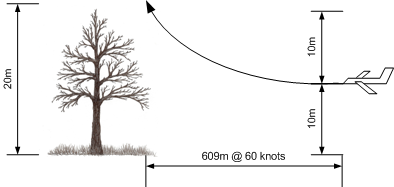
\includegraphics[width=300pt,height=160pt]{./Figures/ProblemStatement.png}
\caption {Case study for obstacle detection requirement}
\label{ob}
\end{figure}

Although digital terrain map are generally available for flight path 
planning and in flight navigation, it does not have the resolution to 
indicate all hazardous obstacle such as tall trees, steep hills, or 
man-made tall objects. The obstacle detection and avoidance system must 
be in place to detect discrete threat, and operate automatically with 
minimum intervene from the operator. 

\section{Contributions}\label{section:Contribution}
The thesis reviews the properties and consistency of a typical Extended 
Kalman Filter (EKF) based SLAM algorithm, and discusses the advantage 
and limitation of vision based SLAM method. The analysis motivates the 
development of an improved method by fusing multiple sensors into a mono 
vision EKF based SLAM framework.

Using a monocular vision for mapping is a bearing only SLAM problem. The 
measurement is through projection, which loses information about the 
relative position of the feature since the range is unknown. Without 
camera motion measurements, map created by monocular vision can be 
scaled arbitrarily. For a SLAM application in aerial scenario, camera 
vibration and sudden movement is common when aircraft is hit by cross 
wind, which can cause the lost of tracked features. A recursive EKF 
based SLAM algorithm is described in this thesis. The method utilizes 
sensor onboard the UAV to provide motion measurement of the camera, and 
improve the robustness of the algorithm under rough flying condition. 
Real aerial data were collected to test the performance and accuracy of 
the algorithm in a scenario similar to the one where the UAV will be 
eventually deployed. The preliminary result of the test flight was 
published in []. This paper is one of the first ones in the field 
that successfully applying monocular vision SLAM in large scale aerial 
application. A more thorough analysis on the behavior of the algorithm 
and its error is presented in this thesis.Furthermore, a number of 
baseline separations for the cameraare tested to optimize the 
performance and computation cost of the algorithm. 

\section{Organization}\label{section:Organization}
The thesis is organized as follows:

\begin{itemize}
\item Chapter 2 presents an overview on sensors, computer vision 
algorithms, SLAM algorithm related to obstacle detection and range 
measurement.
\item Chapter 3 describes the detail implementation of the proposed 
multisensory monocular SLAM algorithm.
\item Chapter 4 describes camera calibration procedure, equipments setup 
for the aerial data collection, and data preparation steps. 
\item Chapter 5 presents detail analysis on the performance of the 
algorithm. Convergence and consistency of the algorithm is discussed in 
section and . Error analysis compared to ground truth data is presented 
in and . The effect of using multiple sensors in improving the 
robustness is discussed in . At last, the camera baseline optimization 
is given in .
\end{itemize}


\chapter{REVIEW ON SENSORS AND RELATED WORK}\label{ch:Review}

\section{SENSORS FOR OBSTACLE DETECTION}\label{sec:sensor}

\subsection{Overview}\label{sec:SensorOverview}

Many work in obstacle detection uses range sensors such as radar, laser 
range finder, LIDAR, sonar. $[$reference goes here$]$. Radar and laser 
range finder provides only point measurement at a given position and 
orientation. To acquire a full 3D range map of a scene, mechanical 
scanning mechanisms are required, which limits the data acquisition rate 
of these device. LIDAR operate in the same manner as laser range finder, 
except with the scanning mechanism built in. These sensors usually have 
high power requirement and mass, and may not be suitable for small and 
mid size UAV. Sonar is usually used in indoor or under water 
applications, and have wide beam profile which make it difficult to 
identify the origin of return signal, and results in low resolution 
range map. 3D flash LIDAR is capable of acquire 3D range measurement 
simultaneously by illuminating the entire field of view of the camera 
with a single laser, and capturing the reflected laser with a 2D imaging 
sensor $[$reference; wikipedia$]$. However, its high cost has limited 
its use in commercial application.

In recent years, many researches use optical sensor as a passive range 
sensor for its low weight, low cost. With the help of computer vision 
technology, optical sensors have been successfully used for range 
mapping and obstacle detection in a number of platforms 
$[$references$]$. There are several types of configuration in using 
optical sensor for range mapping: monocular, binocular, or multi-camera. 
Since optical sensors are bearing only sensors, the principle of range 
measurement is through triangulation a common scene point in two or more 
images captured. For binocular camera setups, two cameras are placed 
apart from each other with their relative geometry known and captures 
images simultaneously. If the position of a scene point can be 
accurately found in the images by both cameras, its distance can be 
calculated by using the difference in position of the projected point in 
images, and the separation of the cameras. 

\begin{itemize}
  \item Radar, sonar, laser range finder, 3D flash lidarvs. optical sensors
  \begin{itemize}
    \item Radar, laser range finder have high power requirement and mass
    \item Depth measurement can be obtained through optical sensors, which 
    are inexpensive and light weight
    \item Depth maps of a 3-D scene can be computed from a single pair of 
    stereo camera. Stereo processing can require significant computational 
    effort
  \end{itemize}
  \item Monocular camera characteristic: 
  \begin{itemize}
    \item bearing-only sensor, which provide the measurement on the 
    direction of the feature, and not the range. Other sensors, such as 
    radar, are range and bearing sensors. 
  \end{itemize}
\end{itemize}

\subsection{Monocular Vision and Binocular Vision}\label{sec:MonoBino}
\begin{itemize}
  \item Optical flow vs. feature detection and tracking
  \item The correspondence problem
  \item Initialization problem (addressed by Inverse depth 
  parameterization)
  \item Lack of scale information of overall map -$>$ must work with other 
  sensors which provide robot motion measurement. 
\end{itemize}

\subsection{Limitation of Optical Sensor in Recursive Algorithm}
\label{sec:OpticalSensorLimitation}

\begin{itemize}
  \item Error Accumulation over Iterations
  \begin{itemize}
    \item Feature quality Decreases over Iterations
  \end{itemize}
\end{itemize}

\subsection{GPS and IMU}\label{sec:gps_and_imu}
GPS and IMU are generally available on UAVs. These sensors provide a 
measurement on the robot motion. Odometry can provide the scale 
information which is missing in the bearing only measurement. 
Furthermore, odometry provides some prior information on the robot 
motion which can help to disambiguate the solution.

\section{SLAM as A Sensor Fusion Framework}
\label{sec:SLAM}
An essential aspect of autonomy for a mobile robot is the capability to 
determine its location. This capability is known as localization. 
Localization is typically a prerequisite for accomplishing real tasks, 
whether it is exploration, navigation toward a known goal, 
transportation of material, construction or site preparation. In many 
applications, the mobile robot has an a priori map. Given a map, the 
robot may localize by matching current sensor observations to features 
in the map. Given enough features and an unambiguous geometry, the pose 
of the robot can be determined or at least narrowed down to a set of 
possible locations.

Usable maps do not always exist, and it is not always possible to have 
accurate externally referenced pose estimates. If an a priori map is not 
available, the robot may need to construct one. With a precise, 
externally referenced position estimate from GPS or similar means, the 
robot can take its sensor observations, reference the observations to 
its current pose, and insert features in the map in the appropriate 
places. Without maps or externally referenced pose information, the 
robot must produce its own map and concurrently localize within that 
map. This problem has been referred to as concurrent localization and 
mapping (CLM) and simultaneous localization and mapping (SLAM).

\subsection{Recursive Probabilistic Estimation using Extended Kalman Filter}
\label{sec:SLAM_using_EKF}

\subsubsection{Kalman Filter}
The Kalman filter \cite{Kalman's original paper}published by R. E.
Kalman in 1960 is a very powerful recursive data processing algorithm
for dynamic stochastic processes. The filter find extensive use in
control and navigation application for its ability of estimating past,
present and even future state. It is an attractive candidate for data
fusion framework as it can process all available measurements
including previous knowledge of the process, regardless of their
precision, to estimate the current value of the variable of interest.
Given a dynamic process that satisfy the assumptions that Kalman
filter is based on, the filter is the optimal algorithm in minimzing
the mean of squared error of the state variable. This section briefly
summerized assumption and formation of Kalman filter that's described
in detail in \cite{from the following}[Sorenson70; Gelb74; Grewal93;
Lewis86; Brown92]. A more intuitive introduction can be found in
chapter 1 of [Maybeck79]
%reference in Welch and bishop
% intro to Kalman filter.

The Kalman filter has three assumptions. 1) The system model is
linear. The linearity is deisred in that the system model is more
esily manipulated with engineering tool. When nonlinearities do exist,
the typical approach is to linearize system model at some nominal
points. 2)The noise embedded in system control and measurement is
white. This assumption implies that the noise value is not correlated
in time, and has equal power in all frequency. 3)The probability
density function (PDF) of system and measurement noise is Gaussian. A
Gaussian distribution is fully represented by the first and second
order statistic (mean and variance) of a process. Most other densities
require endless number of orders of statistic to describe the shape
fully. Hence, when the probability density function of a noise process
is non-Gaussian, the Kalman filter that propagates the first and
second order statistic only include some of the information of the
PDF, instead of all, as would be the case with Gaussian noise.

\paragraph{Kalman Filter Models}
The Kalman filter requires two models. The process model define a
discrete-time controlled process by a linear stochastic difference
equation. The $n\times n$ matrix $A$ relates the state variables
$x_{k-1}$ in previous time step $k-1$ to the state variabl $x_{k}$ in
the current time step $k$. The matrix $B$ relates the optional control
input $\mu$ to the state variables $x$. Given measurement vecor $z_k$
of size $1 \times m$, the measurement model relates the state
variables to the measurements by matrix H of size $n \times m$. The
random variable $w$ and $v$ represent the uncertainty or noise of the
process model, and measurement. $w$ and $v$ are assumed to be
unrelated to each other, and has Gaussian distribution with covariance
$Q$ and $R$. 

\begin{align}
&\text{Process Model: }x_k = Ax_{k-1}+B\mu_{k-1}+w_{k-1}\\
&\text{Measurement Model: }z_k = Hx_k+v_k
\end{align}

\paragraph{The Algorithm}
The Kalman filter operates in prediction and correction cycle after
being initialized \ref{figch2:1}, with the state vector estimate
$\hat{x}^-_k, \hat{x}^+_k$ contains the variable of interest at time
step k, and state covariance matrix $P^-_k, P^+_k$ representing the
error covariance of the estimate. The superscript - indicate the
estimate is a priori (or predicted) estimate, and + indicate the
estimate is a posteriori (or corrected) estimate. The equations used
for prediction and correction are listed in \ref{tab:KF}. In
prediction, an estimate of the state variables are made based on the
known knowledge of the process (the process model). Since there are
always unknown factor not fully described by the process model, the
error of the estimate almost always increase in the prediction. During
correction, a series of calculation were carried out to correct the a
priori estimate. First, the predicted measurement $H\hat{x}^-_k$ are
compared to the new measurement $z_k$. Their difference $z_k -
H\hat{x}^-_k$ is called the measurement innovation, or residual. Next,
the amount of residual is weighted by the Kalman gain $K$, and added
to $\hat{x}^-_k$ as correction. The Kalman gain is fomulated so that
it minimize the a posteriori error covariance matrix $P^+_k$. 

\begin{figure}[h]
\centering
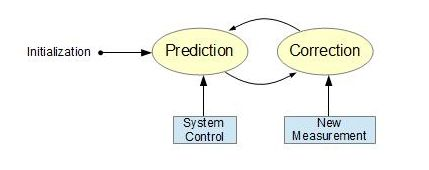
\includegraphics[width=10cm, keepaspectratio=true]{./Figures/KalmanOperation.jpg}
\caption{Kalman Operation Flow Diagram}
\label{figch2:1}
\end{figure}

\begin{table}
\caption{Kalman Filter Operation Equations}
\label{tab:KF}
\centering
\begin{tabular}{|l|c r|}
\hline
\multirow{2}{*}{Prediction} 
& $\hat{x}^-_k=A\hat{x}^+_{k-1}+B\mu_{k-1}$ & \stepcounter{equation}\tetab{\theequation}\\
& $P^-_k = AP^+_{k-1}A^T+Q$ & \stepcounter{equation}\tetab{\theequation}\\
\hline
\multirow{3}{*}{Correction}
& $K_k=P^-_kH^T(HP^-_kH^T+R)^{-1}$  & \stepcounter{equation}\tetab{\theequation}\\
& $\hat{x}^+_k = \hat{x}^-_k+K_k(z_k-H\hat{x}^-_k)$ & \stepcounter{equation}\tetab{\theequation}\\
& $P^+_k = (I-K_kH)P^-_k$ & \stepcounter{equation}\tetab{\theequation}\\
\hline
\end{tabular}
\end{table}
\FloatBarrier

\paragraph{Extended Kalman Filter}
For a discrete-time controlled process, or its relationship with the
measurements are non-linear, a Kalman filter must be linearized about
the estimated trajectory, and is referred to as an extended Kalman
filter or EKF. A process with state vector $x$ and measurement $z$
that is governed by non-linear stochastic difference equation has
process and measurement model 
\begin{equation}
x_k=f(x_{k-1}, u_{k-1}+w_{k-1}),
\end{equation}
\begin{equation}
z_k=h(x_k+v_k),
\end{equation}
\noindent where the random varialbe $w_k$ and $v_k$ represent the
process and measurement noise with variance $Q$ and $R$. The the
Kalman filter operation equations are given in table
\ref{tab:EKF},

\begin{table}[H]
\caption{Extended Kalman Filter Operation Equations}
\label{tab:EKF}
\centering
\begin{tabular}{|l|c r|}
\hline
\multirow{2}{*}{Prediction} 
& $\hat{x}^-_k=f(\hat{x}^+_{k-1},\mu_{k-1},0)$ & \stepcounter{equation}\tetab{\theequation}\\
& $P^-_k = A_kP^+_{k-1}A_k^T+W_kQ_{k-1}W_k^T$ & \stepcounter{equation}\tetab{\theequation}\\
\hline
\multirow{3}{*}{Correction}
& $K_k=P^-_kH_k^T(H_kP^-_kH_k^T+V_kR_kV_k^T)^{-1}$  & \stepcounter{equation}\tetab{\theequation}\\
& $\hat{x}^+_k = \hat{x}^-_k+K_k(z_k-h(\hat{x}^-_k,0))$ & \stepcounter{equation}\tetab{\theequation}\\
& $P^+_k = (I-K_kH)P^-_k$ & \stepcounter{equation}\tetab{\theequation}\\
\hline
\end{tabular}
\end{table}
\FloatBarrier
\noindent where (subscript $k$ omitted)
\begin{itemize}
  \item $A$ is the Jacobian matrix of partial derivatives of $f$ with
  respect to $x$, $$A_{[i,j]}= \frac{\partial f_i(\hat{x}_{k-1}^+, \mu_{k-1},
    0)}{\partial x_j}$$
  \item $W$ is the Jacobian matrix of partial derivatives of $f$ with
  respect to $w$, $$W_{[i,j]}= \frac{\partial f_i(\hat{x}_{k-1}^+, \mu_{k-1},
    0)}{\partial w_j}$$
  \item $H$ is the Jacobian matrix of partial derivatives of $h$ with
  respect to $x$, $$H_{[i,j]}= \frac{\partial h_i(\hat{x}_k^-, 0)}{\partial x_j}$$
  \item $V$ is the Jacobian matrix of partial derivatives of $h$ with
  respect to $v$, $$V_{[i,j]}= \frac{\partial h_i(\hat{x}_k^-,0)}{\partial v_j}$$
\end{itemize}

\noindent Note that when $w$ and $v$ directly describe the noise of
state vector and measurement, the table \ref{tab:EKF} is the same as
table \ref{tab:KF}. 

\paragraph{Tuning}

\subsubsection{Properties of SLAM}
\label{sec:SLAM_properties}

Needs editing.Directly from papers.

Dissanayake proved three important convergency properties of the EKF 
solution to SLAM, namely that: (1) the determinant of any submatrix of 
the map covariance matrix decreases monotonically as observations are 
successively made; (2) in the limit as the number of observations 
increases, the landmark estimates become fully correlated and (3) in the 
limit the covariance associated with any single landmark location 
estimate reaches a lower bound determined only by the initial covariance 
in the vehicle location estimate at the time of the first sighting of 
the first landmark.

The properties imply:

\begin{itemize}
  \item The entire structure of the SLAM problem critically depends on 
  maintaining complete knowledge of the cross correlation between landmark 
  estimates. Minimizing or ignoring cross correlations is precisely 
  contrary to the structure of the problem. (Early EKF for OD work 
  eliminate the cross correlations between features and veichel pose in an 
  attempt to reduce computation complexity.)
  \item As the vehicle progresses through the environment the errors in 
  the estimates of any pair of landmarks become more and more correlated, 
  and indeed never become less correlated.
  \item In the limit, the errors in the estimates of any pair of landmarks 
  become fully correlated. This means that given the exact location of any 
  one landmark, the location of any other landmark in the map can also be 
  determined withabsolute certainty.
  \item As the map converges in the above manner, the error in the 
  absolute location of every landmark (and thus the whole map) reaches a 
  lower bound determined only by the error that existed when the first 
  observation was made (Initialize the parameters using 1st frame as 
  coordinate origin with minimum variance - Algorithm initialization).
\end{itemize}
It is important to note that these theoretical results only refer to the 
evolution of the covariance matrices computed by EKF in the ideal linear 
case. They overlook the fact that given that SLAM is a nonlinear 
problem, there is no guarantee that the computed covariance will match 
the actual estimation erros which is the true SLAM consistency issue. 

\subsubsection{Linearization Error and Consistency}
\label{sec:Linearization_error_and_consistency}

Many research report filter divergence due to linearization error. 
Literature review here:
% the citation is a paper that cited the definition from a book.
As defined in \cite{Huang_2008}, a state estimator is consistent
if the estimation errors (i) are zero-mean, and (ii) have
covariance matrix smaller or equal to the one calculated by the filter.

Huang investigate further on properties and consistency of nonlinear 
two-dimentional EKF based SLAM problem, and conclude:

\begin{itemize}
  \item Most of the convergence properties in $[$3$]$ are still true for 
  the nonlinear case provided that the Jacobians used in the EKF equations 
  are evaluated at the true states.
  \item The main reasons for inconsistency in EKF SLAM are due to (i) the 
  violation of some fundamental constraints governing the relationship 
  between various Jacobians when they are evaluated at the current state 
  estimate, and (ii) the use of relative location information from robot 
  to landmarks to update the absolute robot and landmark location 
  estimates.
\end{itemize}

The robot orientation uncertainty plays an important role in both the 
EKF SLAM convergence and the possible inconsistency. In the limit, the 
inconsistency of EKF SLAM may cause the variance of the robot 
orientation estimate to be incorrectly reduced to zero.

Linearization error can be interpreted as error resulted from 
calculating the Jacobian at the estimated state (wrong state) instead of 
the true state. 

\subsubsection{Camera Centric Coordinate System}
\label{sec:cam_centric}

\subsubsection{SLAM for Large Scale Maps}

%%% Local Variables:
%%% mode: latex
%%% TeX-master: "thesis"
%%% End:


%\newchapter{chapter3}
\chapter{Experiments with Real Aerial Data}
\section{Equipment Setup and Flight Data Collection}
% word checked.
The biggest contribution of the project is that the proposed algorithm
was tested and proven feasible with real flight data collected by the
author. The aerial video and navigation data were collected through a
survey flight with the support of Sander Geophysics Ltd. A main
purpose of the test flight was to obtain aerial video with the camera
close to the ground to mimic the scenario of a low flying UAV. This is
difficult to achieve with any manned fixed wing aircraft since terrain
following flight at low altitude is very dangerous. Therefore, a
helicopter was used to conduct the survey flight to achieve the
terrain following action. To get sensors close to the ground and to
allow for flexible sensor mounting, a simulated unmanned aircraft
system (SUAS) was used to carry all sensors. The SUAS was towed by a
helicopter via a tow rope of 33 meters length (Figure
\ref{fig:towedSUAS}). Yet, sufficient clearance must be established
between the SUAS and the vegetation to prevent the SUAS from being
caught by tree branches. As a result, the helicopter flew a planned
path at approximately 100 meters above ground, and the SUAS was at
approximately 70 meters above ground.

\begin{figure}[h]
\centering
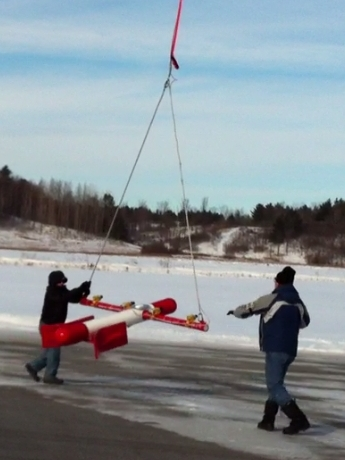
\includegraphics[width=6cm,keepaspectratio=true]{./Figures/SUAS_TAKEOFF2.jpg}
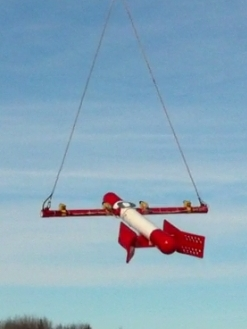
\includegraphics[width=6cm,keepaspectratio=true]{./Figures/SUAS_TAKEOFF3.jpg}
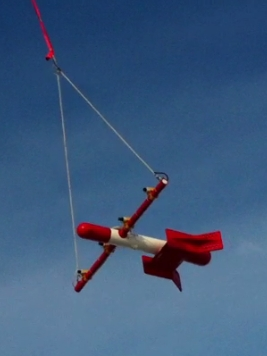
\includegraphics[width=6cm,keepaspectratio=true]{./Figures/SUAS_TAKEOFF4.jpg}
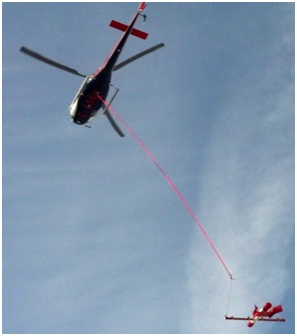
\includegraphics[width=6cm,keepaspectratio=true]{./Figures/towed_SUAS.jpg}
\caption{SUAS towed by a helicopter}
\label{fig:towedSUAS}
\end{figure}
\FloatBarrier

Sensors mounted on the SUAS (Figure \ref{fig:SUAS}) included one wide
angle CCD camera with 6mm focal length lens capturing monocular image
sequences at 30 frames per second, a pair of narrow angle CCD cameras
for binocular image sequences, a GPS antenna, a three-axes fluxgate
sensor, and Athena GS-111m, a flight control INS/GPS navigation unit
\cite{_athena_????} which captures vehicle velocity, acceleration,
rotation, altitude. Analog video and navigation data were sent to the
helicopter via three BNC cables and one data cable for recording.
Installed in the helicopter were two SGL data acquisition systems,
named CDAC. This system records video and navigation data from the
SUAS, as well as data from sensors installed on the helicopter,
including GPS, radar altimeter, laser altimeter, air pressure,
temperature, humidity, etc. (Figure \ref{fig:CDAC}). Videos from the
three cameras were digitized to a resolution of 720 pixels by 480
pixels using three Parvus MPEG4 video encoders installed in the CDACs.
Videos were time-stamped with GPS second on the image screen (Figure
\ref{fig:video_snapshot}) for post-flight synchronization with the
navigation data. Because the test flight recorded data from all
available sensors on board the SUAS and the helicopter, these
recordings would still be useful should any future research require
more sensor data.

\begin{figure}[h]
  \centering
  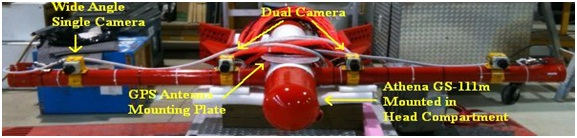
\includegraphics[width=14cm,keepaspectratio=true]{./Figures/SUAS.jpg}
  \caption{Sensors mounting location on SUAS}
  \label{fig:SUAS}
\end{figure}

\begin{figure}[h]
  \centering
  \includegraphics[width=6cm,keepaspectratio=true]{./Figures/athena.jpg}
  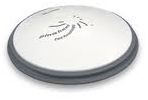
\includegraphics[width=6cm,keepaspectratio=true]{./Figures/GPS_antenna.jpg}
  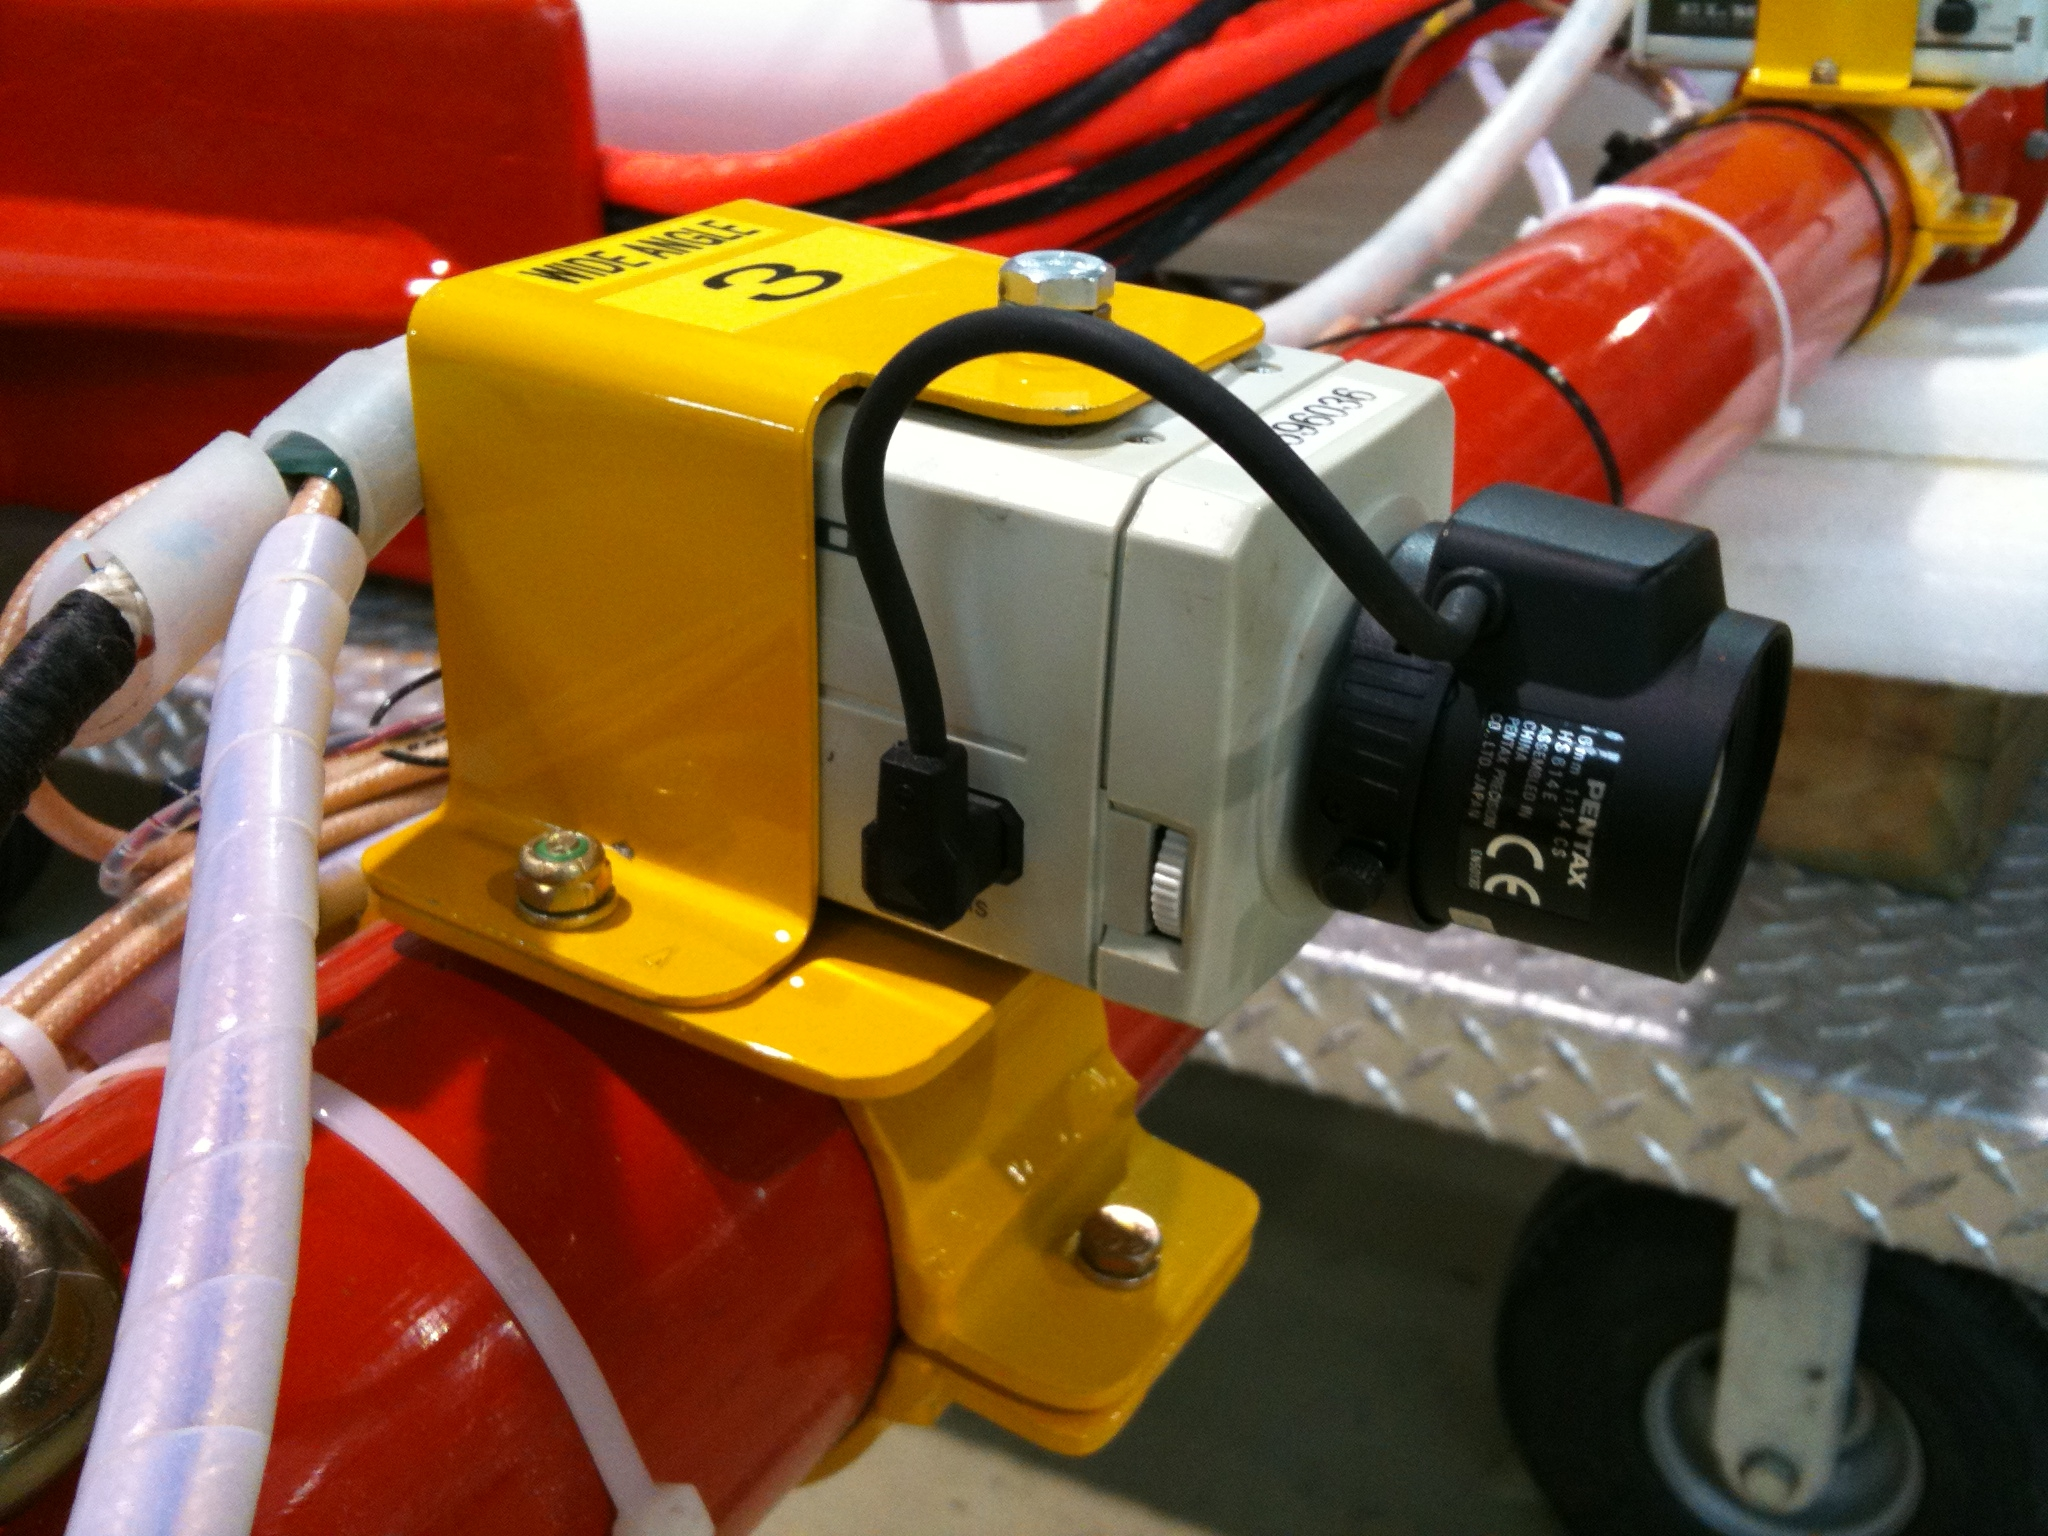
\includegraphics[width=10cm,keepaspectratio=true]{./Figures/wide_cam.jpg}
  \caption{Sensors mounted on SUAS. Top left: Athena
  GS-111m, top right: GPS antenna, bottom: monocular CCD camera}
  \label{fig:SUAS_sensors}
\end{figure}

\begin{figure}[h]
  \centering
  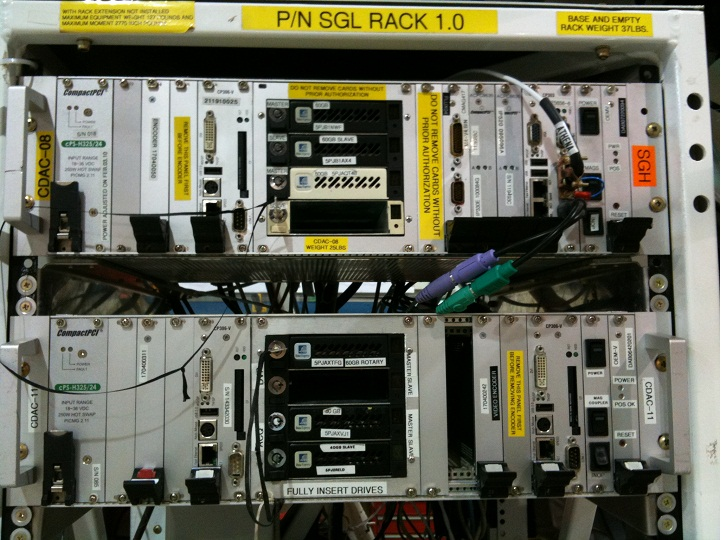
\includegraphics[width=12cm,keepaspectratio=true]{./Figures/CDAC_Rack.jpg}
  \caption{Compact PCI data acquisition system (CDAC)}
  \label{fig:CDAC}
\end{figure}

\begin{figure}[h]
  \centering
  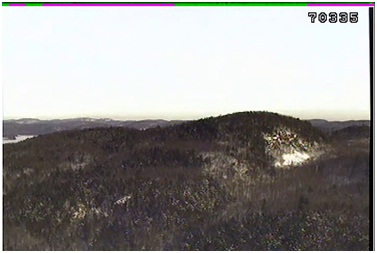
\includegraphics[width=12cm,keepaspectratio=true]{./Figures/video_snapshot.jpg}
  \caption{Image from monocular camera with GPS second timestamp}
  \label{fig:video_snapshot}
\end{figure}

\FloatBarrier

\section{Camera Calibration}\label{sec:camcal}
% word checked
Camera calibration decodes the relation between image pixels and the
actual 3D world. The intrinsic parameters could be affected by a
number of environmental conditions, such as temperature, and humidity.
To extract the camera parameters at a camera condition as close as
possible to the one during test flight, camera calibration was
performed right after the SUAS returned to the SGL hanger. A camera
calibration was done by taking a video of a checkerboard pattern with
various translations and rotations from the camera. A total of 20 views
of the calibration target were chosen from the video, and fed to the
calibration algorithm. A few examples are shown in Figure
\ref{fig:camcal}.

\begin{figure}[h]
  \centering
  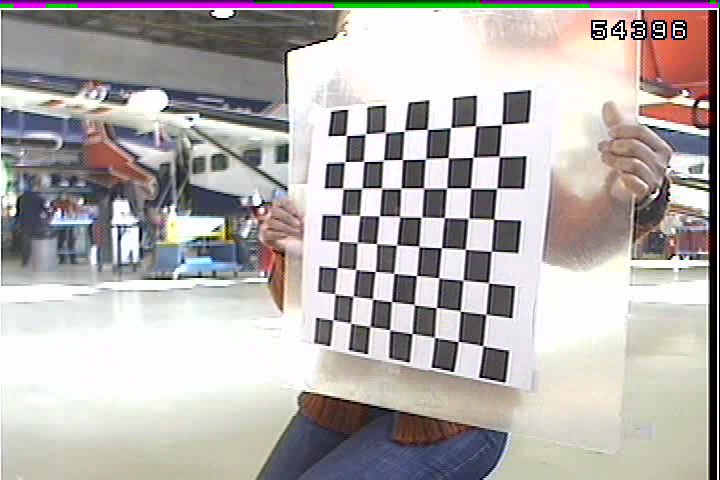
\includegraphics[width=4cm,keepaspectratio=true]{./Figures/camcal/camcal1_130.jpeg}
  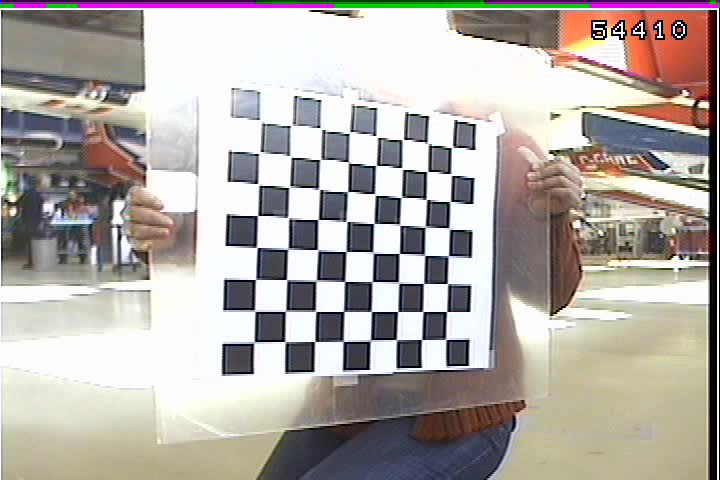
\includegraphics[width=4cm,keepaspectratio=true]{./Figures/camcal/camcal1_140.jpeg}
  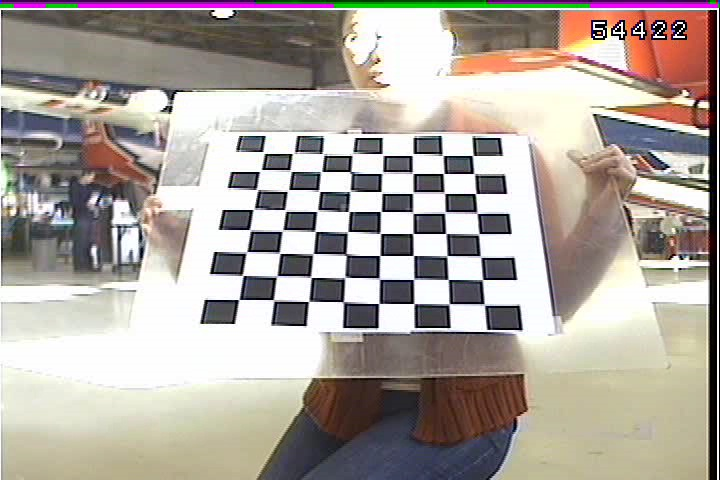
\includegraphics[width=4cm,keepaspectratio=true]{./Figures/camcal/camcal1_160.jpeg}
  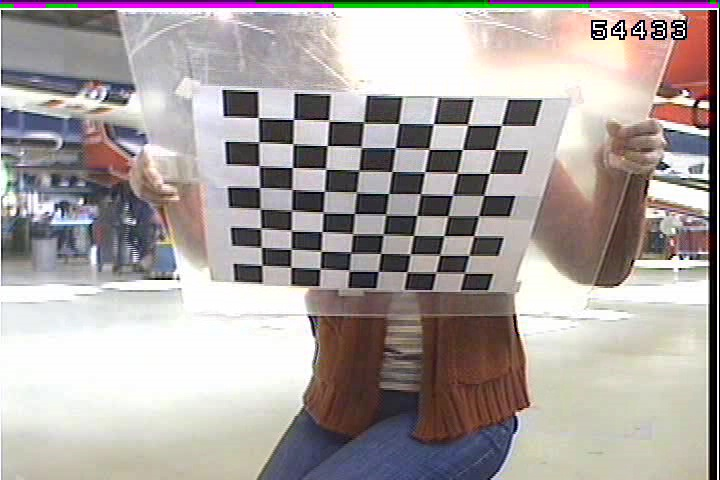
\includegraphics[width=4cm,keepaspectratio=true]{./Figures/camcal/camcal1_180.jpeg}
  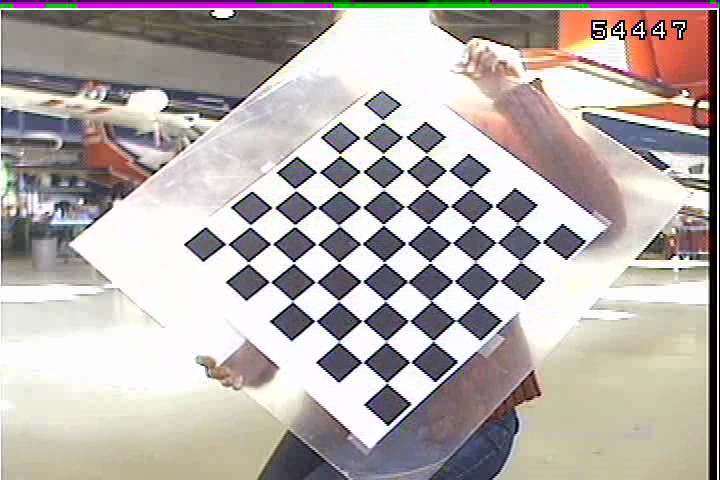
\includegraphics[width=4cm,keepaspectratio=true]{./Figures/camcal/camcal1_210.jpeg}
  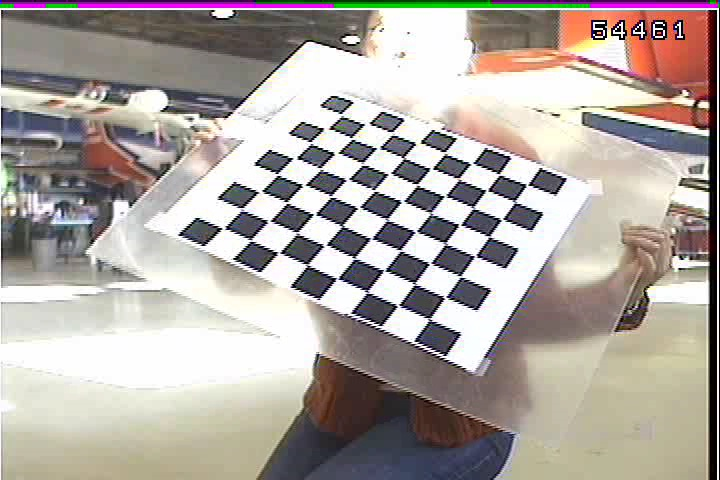
\includegraphics[width=4cm,keepaspectratio=true]{./Figures/camcal/camcal1_240.jpeg}
  \caption{A subset of camera calibration input images}
  \label{fig:camcal}
\end{figure}

The program ``calibration.exe'' was used to calibrate the camera. This
program came with the OpenCV installation. The digitized images have a
resolution of 720 pixels in width and 480 pixels in height. Table
\ref{tab:camcalresult} below lists the calibration results.

\begin{table}[h]
\caption{Camera calibration result}
\label{tab:camcalresult}
\centering
\begin{tabular}{|c|c|}
\hline
Parameter & Result\\ \hline
$f_x$ & 887.6 pixels \\ \hline
$f_y$ & 805.7 pixels\\ \hline
$c_x$ & 381.8 pixels\\ \hline
$c_y$ & 293.7 pixels\\ \hline
$k_1$ & -0.102 \\ \hline
$k_2$ & -0.535 \\ \hline
$p_1$ & 1.15e-003 \\ \hline
$p_2$ & 8.40e-003 \\
\hline
\end{tabular}
\end{table}
\FloatBarrier

\section{Ground Truth Data Collection}
The localization ground truth was obtained through the flight
control unit GS-111m on board the SUAS. The unit recorded the SUAS
position in GPS longitude and latitude coordinates. Orientation was
obtained from the roll pitch and heading measurements. Roll and pitch
accuracy has $0.1^\circ$ and $0.1^\circ$ standard deviation.
Heading accuracy can achieve $0.5^\circ$ \cite{_athena_????}.

Landmark position ground truth came from a digital elevation map (DEM)
downloaded from the CGIAR-CSI website \cite{_cgiar-csi_????}. The DEM
contains longitude, latitude and sea level elevation of the terrain
with a resolution of approximately 100 meters by 100 meters. 

%consider adding the ground truth DEM figure here. 


%%% Local Variables:
%%% mode: latex
%%% TeX-master: "thesis.tex"
%%% End:

\chapter{Result From Flight Data}\label{ch:FlightResult}

This chapter is divided into three main sections. Firstly, the
algorithm's convergence and consistency was analyzed. Secondly, the
accuracy of the algorithm is examined by comparing to ground truth
data. The third section summarized test results for tuning the
algorithm for better accuracy and efficiency. The forth section
present the advantage of using IMU data. The fifth section outline
the inadequacies of the CC\_EKF\_SLAM algorithm identified.

To test the performace of CC\_EKF\_SLAM algorithm, 4 segments of video
were selected from the test flight video, and 400 frames were
processed in each piece. The filter initialized 40 features at the
first frame, and maintain the tracked features amount at this number
by initializing new features when existing features moved out of FOV.

Since all parameters are tracked in camera frame, their value is 
different when viewed from a fixed point in world frame. Therefore, all 
parameters are converted back to world frame before plotting. 

\section{Convergence and Consistency}

\subsection{Convergence and Tracking}
Among the feature parameters, the feature initialization point were
initialized to the zero which is the origin of the camera centric
coordinate. $\phi$ and $\theta$ were calculated directly from the
feature position on image plane, have high accuracy and don't require
convergence. The only parameter that goes through a converging process
is the features' inverse depth $\rho$, which were initialized to 0.1
for all features. Figure \ref{fltfig:1} shows the $1/\rho$ plot for
video segment1 over 200 frames. The depth estimators went through
rapid changes for several frames after their initialization. Within
approximate 20 frames, most estimtors settles to a stable value. The
estimated features distance ranged from 400 meters to about 1500
meters, confirming the algorithm's capability for estimating features
at great distance. On the other hands, some features take a long time
to settle, such as feature 9, 27, ??, while some other never settled,
such as 12 and 20.
% is the non and slowly settled feature has any character in its
% pattern? ie. is a line feature, instead of corner? A outlier filter
% should be in place to get rid of the poor features (future work).

\begin{figure}[h]
\centering
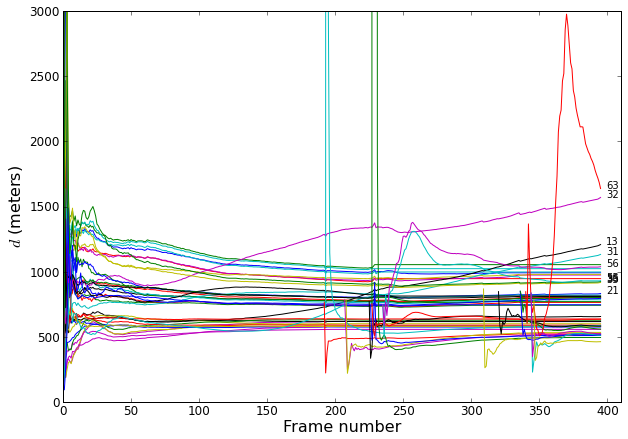
\includegraphics[width=10cm, keepaspectratio=true]{./Figures/fltfig/cut1/Figure10.png}
\caption{Inverse Depth Convergence}
\label{fltfig:1}
\end{figure}

Although the features initialization point $[x_i, y_i, z_i]$, and the
deviation-elevation angle pair $[\phi, \theta]$ did not go through a
converging stage, they do get updated and converted into the new
camera coordinate using the estimated camera motion at every
iteration. As a result, the accuracy of these parameters varies.
Ideally, the coordinates should converge to a fixed value. However,
the plot indicates a variation as the vehicle travels along. Figure
\ref{fltfig:2} shows the tracking of these parameters over the entired
processed frames.
These parameters were stable for about 200 frames. As soon as any
feature was deleted from the filter and new features added, the
paramters of the feature after being converted into world
frame start to drift. In \ref{fltfig:2} the deletion of old feature is
marked by a vertical gray dash line. It shows that the parameters of
the deleted feature start to drift right after that line. The $y_i$
and $z_i$ are most affected. The behavior is caused by the estimated
error in the SUAS localization. In order to compensate the error in
localization(Figure \ref{fltfig:4}), the algorithm made adjustment on the
estimate of  features parameters so that the combinational result
agrees with the measurement. On the other hand, features mapping is
not affected too much by the error in localization. Because their
parameters are transformed in each iteration to the new camera frame
using the estimated SUAS motion which carries the error. As long as
their paramters are updated together with the estimated motion on that
iteration, and transformed back to the world frame using the same
estimated motion, the final result of features location in world frame
is inaffected by the error in the SUAS localization. However, for
feature removed from the filter, their parameters are no longer
updated, therefore revealing the error in SUAS localization. 

\begin{figure}[h]
\centering
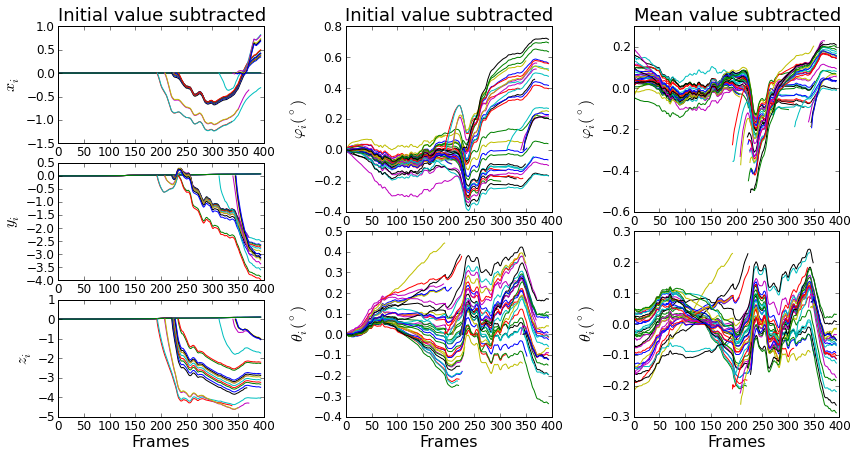
\includegraphics[width=12cm, keepaspectratio=true]
{./Figures/fltfig/cut1/Figure20.png}
\caption{Feature parameters tracking}
\label{fltfig:2}
\end{figure}

\subsection{Consistency Analsysis}
A EKF system becomes inconsistent when the variance of state vector
element becomes too small and forbid an effective update. In addition,
the uncertainty of the SUAS position should increases as it move away
from the origin. To examine the consistency of the CC\_EKF\_SLAM
algorithm, the variance of all state vectors for all procesed frames
were extracted and plotted in figure \ref{fltfig:3}. The two plots on
the left shows the variance of world frame position and orientation in
camera frame. The three plots on the right show the variance of
feature parameters. The variance of world frame position increases
with iterations. On the other hand, world frame orientation decreases
with iterations. Especially the orientation in Y and Z axis remain
below 5e-7 for the most time. For feature parameters, all variance
decreases with iterations, and their value is very small. 
\begin{figure}[h]
\centering
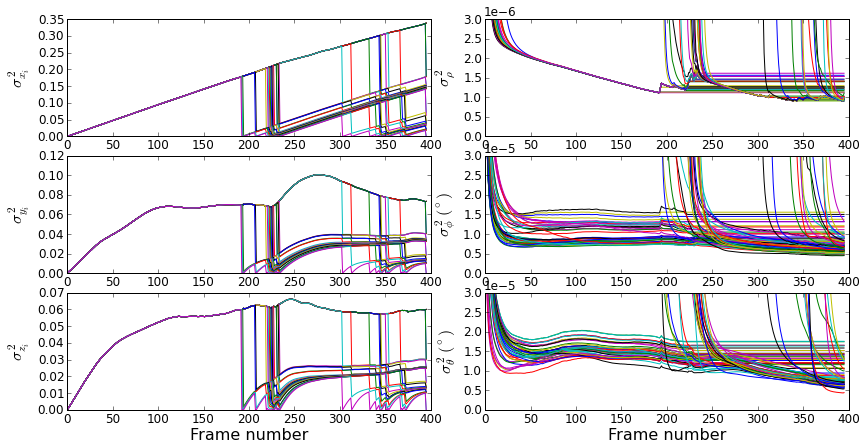
\includegraphics[width=12cm, keepaspectratio=true]
{./Figures/fltfig/cut1/Figure40.png}
\caption{State vector variance}
\label{fltfig:3}
\end{figure}

To see how variance affect the correction the filtered made on the
state vector, the correction applied each iteration were plotted ni
figure \ref{fltfig:4}. The $1^{st}$ column shows the correction on
world frame position in camera frame. The $2^{nd}$ column shows the
correction on feature initialization coordinate in camera frame. The
$3^{rd}$ column shows the correction on features parameters $\rho$,
$\phi$ and $\theta$. It can be observed that world frame position on Y
and Z component receive more correction than the X component, despite
their variance is smaller than the X axis. Similarly, feature
parameter $\theta$ and $\phi$ receive more correction than $\rho$
despite their variance is smaller than the variance of $\rho$.
Secondly, there is a strong inverse correlation between the Y and Z
component of feature initialization position and the world frame
position on Y and Z axis. Similarly, $\phi$ is correlated to world
frame position Z component, $\theta$ is correlated to the world frame
position Y component. Since the features initialization coordinate has
high correlation with the world frame Y and Z position, the main
contributor all the drift comes from the world frame position
correction. Figure \ref{fltfig:5} shows the Kalman Gain over the 5
iteration for the first 35 elements in the state vector, which include
world frame parameters, SUAS motion parameters, and parameters for the
first 4 features. At $1^{st}$ iteration, the high gain is on the
feature parameter $\rho$. Starting from the $2^{nd}$ iteration, more
and more weight goes into the Y and Z component of world frame
position, as well as the Y and Z component of features initialization
position. Although the variance of these two parameters is small, it
is possible that the linearization of the measurement model increased
the correction gain on these parameter. This issue requires further
digging, and will be analyze as a future work.  

\begin{figure}[h]
\centering
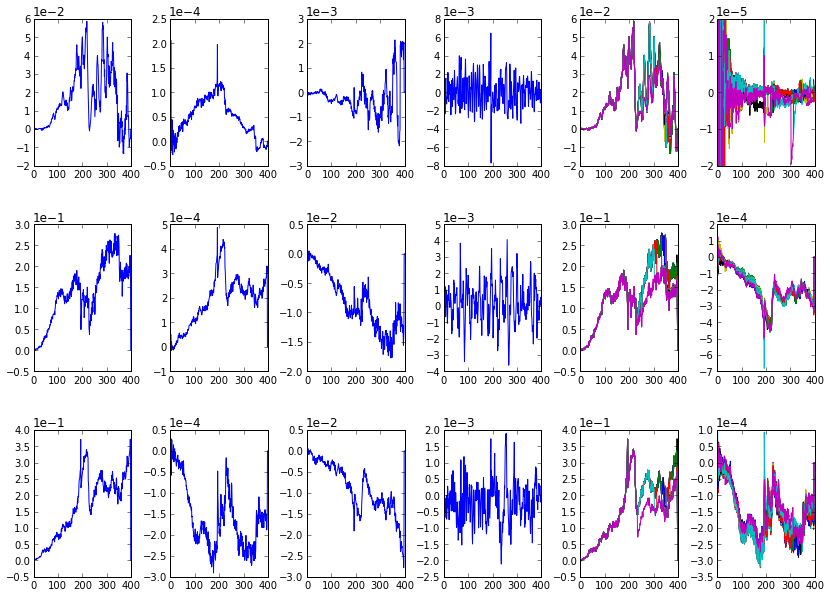
\includegraphics[width=12cm, keepaspectratio=true]
{./Figures/fltfig/cut1/Figure112.png}
\caption{State Vector Corrections}
\label{fltfig:4}
\end{figure}

\begin{figure}[h]
\centering
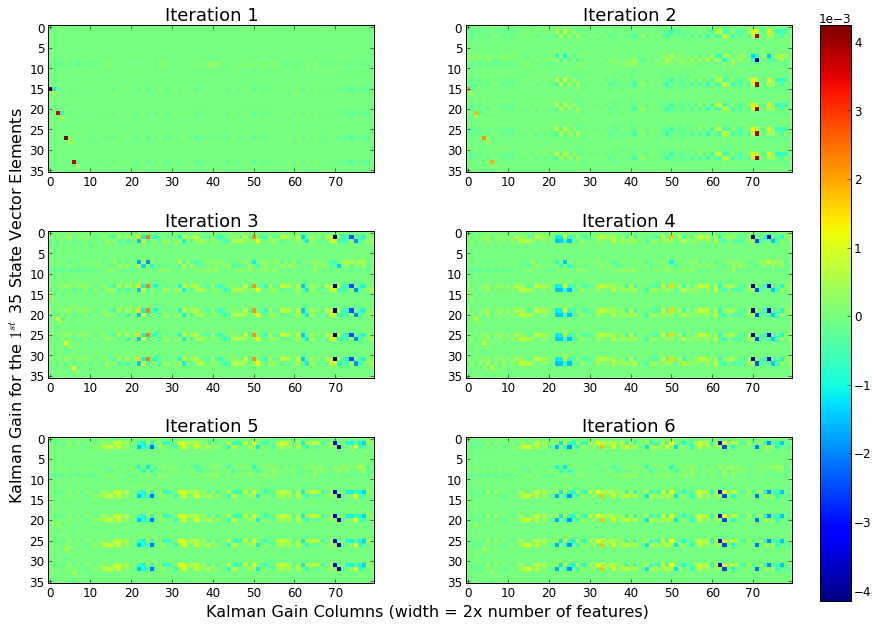
\includegraphics[width=14cm, keepaspectratio=true]
{./Figures/fltfig/cut1/Figure113.png}
\caption{Kalman Gain Matrix for the first 35 State Vector Elememts}
\label{fltfig:5}
\end{figure}

In summary of the consistency analysis, the filter has not moved into
inconsistent state at 400 iterations. However, the variance of
parameters does decrease at each iteration that it is only a matter of
time that the filter will become inconsistent. Therefore, the filter
will require a reset procedure to 

\begin{enumerate}
  \item Resync the SUAS location with GPS. 
  \item Reset its covariance matrix. 
\end{enumerate}

\noindent for any large area operation. 

\section{Accuracy}
\subsection{SUAS Localization}

The SUAS location and orientation were verified in UTM coordinate.
Ground truth data comes from the GPS for position, and magnetometer
for orientation. The GPS positioning can generally achieve 7.8 meters
in accuracy \cite{GPS_ACCURACY}. For orientation, accuracy on the
datasheet specified $0.1^{\circ}$ for roll and pitch, and
$0.5^{\circ}$ for heading. Figure \ref{fltfig:6} shows the estimated
SUAS position and orientation, groundtruth data, and the error. From
the comparison, X position error reached 20m maximum, while Y and Z
position error is bigguer, reaching 50 meter and 30 meters respectly.
For orientation, the etimated value agrees with the ground truth
pattern, with maximum error within 0.02 rad or $1.15^{\circ}$.
Although the error of pitch is biased to the negative side, and error
of heading is biased to the positive side. there was not sign of error
diverging within the 400 frames procesed.

\begin{figure}[h]
\centering
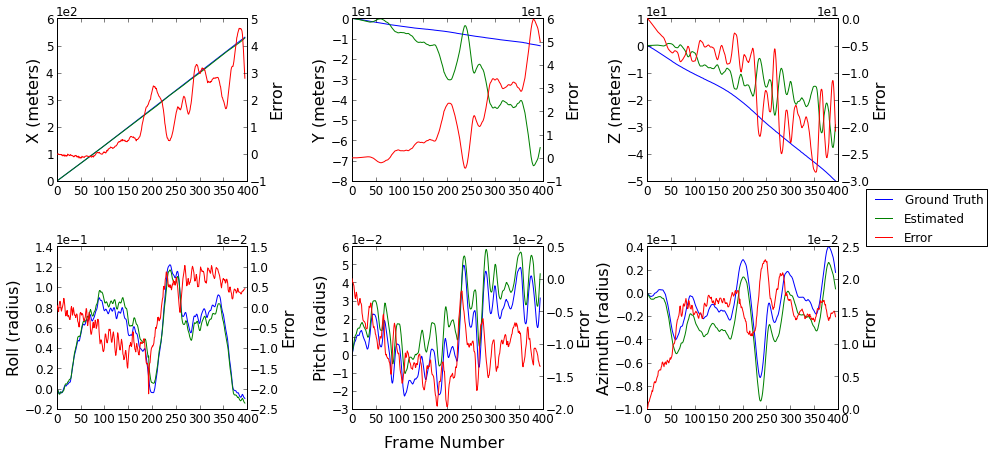
\includegraphics[width=12cm, keepaspectratio=true]
{./Figures/fltfig/cut1/Figure30.png}
\caption{SUAS position and orientation}
\label{fltfig:6}
\end{figure}

\subsection{Features Mapping}

Although raw ground truth data for the terrain was downloaded from
\cite{_cgiar-csi_????} CGIAR-CSI website, making data correspondence
with the estimated feature is non-trival for natual scene where it
lacks of signature landmark sucn as building corners. From the
experience of analyzing simulation data (chapter 6), the initialized
feature deviation and elevation angle $\phi$ and $\theta$ agrees very
well to the ground truth value. In addition, feature initialization
position is set to $[0, 0, 0]$ in camera frame, therefore carris no
error. Therefore, the following procedure are used the find the
corresponding ground truth location for any estimated feature. 

\begin{enumerate}
  \item The frame number at which feature was initialized was
  identified, and ground truth location of the SUAS at that frame was
  recorded.
  \item Shift DEM to the initialization point using the SUAS ground
  truth location recorded
  \item Align the feature deviation $\theta$ and elevation $\phi$ angle to UTM frame.
  (These angles were recorded in camera frame)
  \item Create a vertical plane using $\theta$ and slice the DEM to
  form a 1D elevation plot (Figure \ref{fltfig:7} blue line)
  \item Create a line using $\phi$ and intersect the 1D elevation plot
  (Figure \ref{fltfig:7} green line). The $1^{st}$ intersection point
  is used as ground truth feature location.
\end{enumerate}

\begin{figure}[h]
\centering
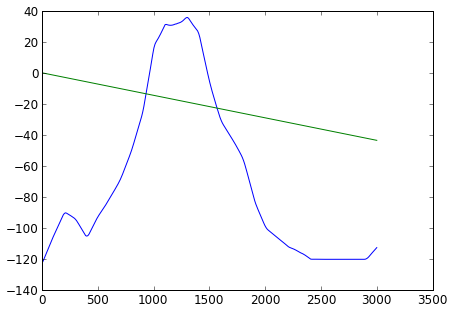
\includegraphics[width=12cm, keepaspectratio=true]
{./Figures/fltfig/cut1/intersect0_0.png}
\caption{Feature position error}
\label{fltfig:7}
\end{figure}

By comparing to the ground truth feature location extracted using the
method describe above, figure \ref{fltfig:8} shows the feature
position error convergence plot in world frame. Feature locations are
compared in world frame for the ease of corresponding the estimated
features and terrain plot with the video by eye. The error convergence
is plotted in figure \ref{fltfig:8} top left. X component (along which
axis the SUAS is traveling) of feature position converge to near zero
in general with maximum error less than 120m for the converged
features. Y component shows a clear offset for features not
initialized at first frame. This behavior is similar to what's seen in
the simulation analysis \ref{section?} where offset in features
position estimates are caused by drift in SUAS localization
estimation. In this case, the features position were converted into
world frame using the the estimated SUAS position, while the ground
truth feature positio are found using the ground truth SUAS position,
which is different than the estimated. Therefore the offset error can
be seen. Z component does not show such offset, but some features' Z
component position drift away after new features were added into the
filter. This drift could be related to the drift in estimates of angle
$\phi$ (figure \ref{fltfig:2}).

\begin{figure}[h]
\centering
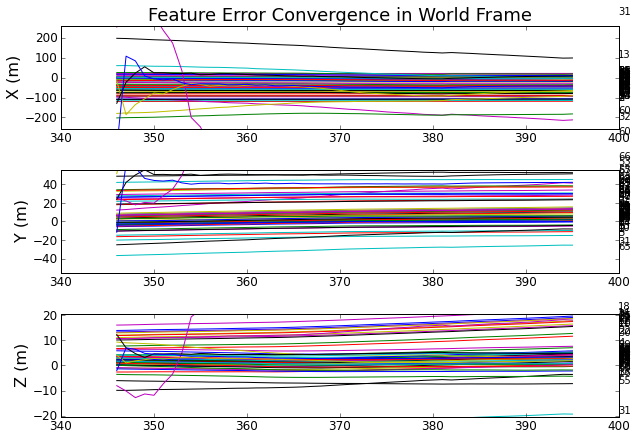
\includegraphics[width=7cm, keepaspectratio=true]
{./Figures/fltfig/cut1/Figure50.png}
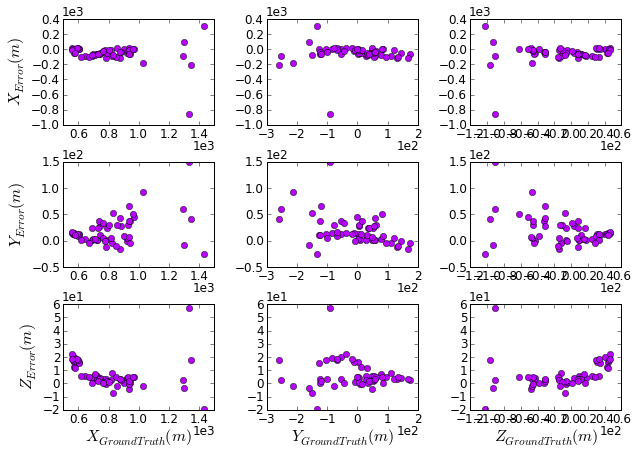
\includegraphics[width=7cm, keepaspectratio=true]
{./Figures/fltfig/cut1/Figure80.png}
\caption{Left: , right: }
\label{fltfig:8}
\end{figure}

Plotting the actual estimated and ground truth features position
reveals relation between the error and the feature's position. Figure
\ref{fltfig:9} bottom plots the feature positions and error at frame
398. First on X axis, the biggest error occur on feature number 65
which is initialized pretty late in the sequence, and has not
converged properly. On Y axis, the position plot also shows feature
number higher than 40 carries an offset error. In addition, the
average error is increasing as feature number gets bigger, which
indicate the further the feature initialization point is from the
world origin, the bigger this offset error will me. On Z axis, besids
the feature 65 carries a big error, features with ground truth Z
position bigger than 25 generally has an error of 15-20 meters. If the
error are plotted against the ground truth position (figure
\ref{fltfig:8} right), it can be seen that these features all
located within 600 meters to the camera. 

\begin{figure}[h]
\centering
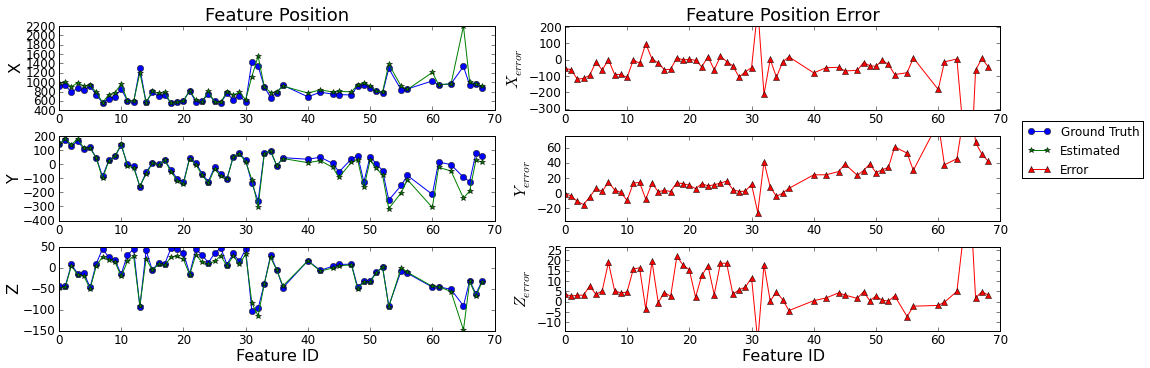
\includegraphics[width=14cm, keepaspectratio=true]
{./Figures/fltfig/cut1/Figure60.png}
\caption{Feature position and error. Left: , right: }
\label{fltfig:9}
\end{figure}

Using the estimated feature position, a terrain map can be generated.
Figure \ref{fltfit:10} shows the terrain map generated from the
feature position analyzed above. On the right, the ground truth DEM is
also shown for comparison. 

\begin{figure}[h]
\centering
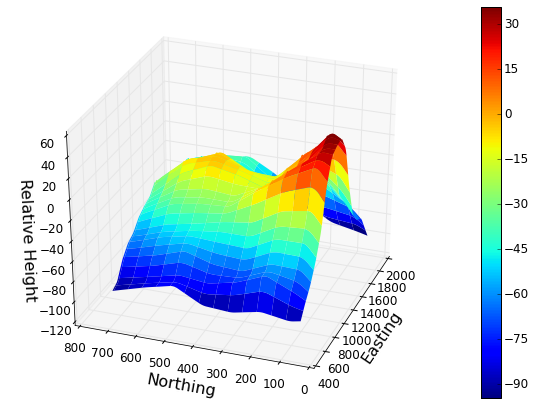
\includegraphics[width=7cm, keepaspectratio=true]
{./Figures/fltfig/cut1/Figure90.png}
\caption{Terrain map. Left: estimated, right: ground truth }
\label{fltfig:10}
\end{figure}


%%% Local Variables:
%%% mode: latex
%%% TeX-master: "thesis"
%%% End:

\chapter{Error Analysis via Simulation}\label{ch:simulation}
There are many factors impacts the accuracy in UAS localization and 
feature position estimation, and they can be sorted into three main 
categories: 

\begin{enumerate}
  \item Noise in system intrinsic parameters. The system intrinsic
  parameters includes
  \begin{itemize}
    \item Camera intrinsic parameters
    \begin{itemize}
      \item Coordinate of optical center on image plane $[c_{x}, c_{y}]$
      \item Scaling factor to project feature in 3D world to image
      plane $ [f_{x}, f_{y}]$
      \item Lens distortion parameters $[k_{1}, k_{2}, p_{1}, p_{2}]$
    \end{itemize}
    \item Image resoluttion.
    \item Accelerometer bias 
  \end{itemize}
  \item Error introduced by LK tracking algorithm. Reliable vision
  tracking is an entire field of research in itself. Pyramid
  implementation of Lucas-Kanade (LK) tracking is used in this work,
  and there are a number of factors contribute to its performance.
  Firstly, LK tracking algorithm tracks features by comparing the
  intensity of a window of the image centered at the feature
  coordinate in image from one frame to another. The searching process
  terminates when the sum of error on the windowed image intensity is
  lower than a value set by user, or when iteration of search has
  reached a maximum number set by user. Secondly, as scene evolve from
  frame to frame, the initial feature appears differently from frame
  to frame as the viewing distance and angle is different. Thirdly,
  sudden intensity change in the image sequences significant noise in
  the tracking. In outdoor setting, intensity change can be introduced
  by many factors, such as changes of sky area in a image, sun glare,
  UAV enters or exits cloud shades, or camera auto-adjust its shuttle
  speed, etc.
  \item Error caused by the SLAM algorithm itself. The algorithm
  estimated features coordinate through a model that represents the
  relation between UAS location, feature location and UAS motion. As
  the model is non-linear, the linearization process introduces error
  into the result.
\end{enumerate}

To better understand the impact of the factors listed above. A 
simulation is performed to examine the impact item 1 and item 3. 

The simulator first generates a 3D point cloud ranging from 100 meters 
to 3000 meters from the camera. At each frame, the coordinates of the 3D 
points are first transformed to the new camera frame using the measured 
UAS motion. Next, the 3D points are projected to the image plane using a 
camera model defined by $[c_{x}, c_{y}, f_{x}, f_{y}, k_{1}, k_{2}, 
p_{1}, p_{2}]$, and digitized to a resolution of choice. 

\section{An Ideal Case}
First of all, understanding the algorithm's performance under no noise, 
or nearly no noise condition provide a solid ground for the analysis 
later on. This simulation shows how much error the model itself 
generates under the most basic flying condition, which is moving forward 
at constant speed. The low noise environment is configure as such,

\begin{itemize}
  \item UAS is moving forward (X axis) with constant speed at 60 knots. 
  \item Y axis and Z axis translational movement are limited to white
  noise with standard deviation of 0.08 meters and a mean of 0.
  \item UAS rotation are modelled by white noise with standard
  deviation of 0.01 degree and a mean of 0
  \item No error was introduced due to image digitization. (i.e. the
  projected feature position on image plane was not digitized to any
  sensor resolution)
  \item No error was introduced from camera model mismatch. (i.e.
  camera model used by simulator is exactly the same as the one used
  by CC\_EKF\_SLAM algorithm.
\end{itemize}

\subsection{UAS Localization}
The estimation of UAS coordinate and orientation is first analyzed, as 
these estimates are directly used to perform transformation between 
camera and world frame. Figure \ref{fig:simfig1} plots the UAS 
translation and rotation against video frame number. The ground truth 
and estimated value are plotted in blue and green lines respectively. 
The error defined by $Estimated-Ground Truth$ is plotted in red line. 
Under a simple forward only motion, the algorithm tracked the UAS status 
quite well, with error on translational motion less than 1 cm and error 
on rotational motion less than 3e-3 degree. 

\begin{figure}[h]
\centering
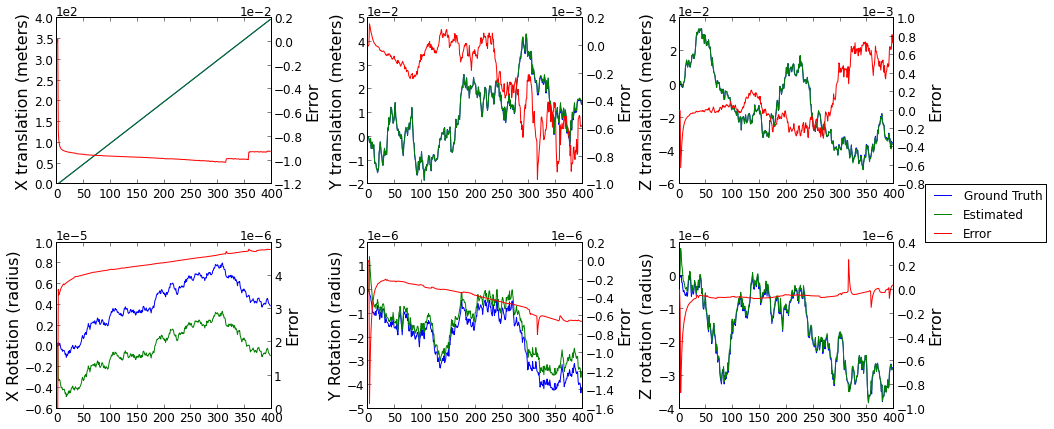
\includegraphics[scale=0.3]{./Figures/SimulationFigures/Figure1.png}
\caption{UAS localization error under no noise condition}
\label{fig:simfig1}
\end{figure}


\subsection{Features Mapping - Convergence and Accuracy}

Figure \ref{fig:simfig5-8} left shows feature parameters $[d, \varphi
,\theta]$ (where $d=1/\rho $) plotted against frame number for the
first 50 frames. The feature depth $d$ for all features converged
within 3 frames; elevation-azimuth angles $[\varphi ,\theta]$ stay
almost constant after initialization. A more detail graph can be seen
from the error convergence plot for these parameters (Figure
\ref{fig:simfig5-8} right.) which shows the tracking error of these
parameters for 400 frames. The error of feature distance$ d$ continues
to approach zero as the tracking continues. $[\varphi ,\theta]$ show
small drift within $+/-0.0002^{\circ}$ respectively. However, as
tracking continue into later frames, error of $[\varphi ,\theta]$
gradually grew bigger. The resulting error for feature coordinate in
world frame represented in standard Euclidean XYZ parameterization is
plotted in ??. The features positions errors in world frame converge
to zero as tracking continues. During the process, certain features
moved out of the FOV, and therefore its position estimation remained
unchanged since then. At the end of the 400 frames, the x axis
position error of the feature reduced to +/-0.2 meters; y and z axis
error reduce to +/-0.02 meters

\begin{figure}[h]
\centering
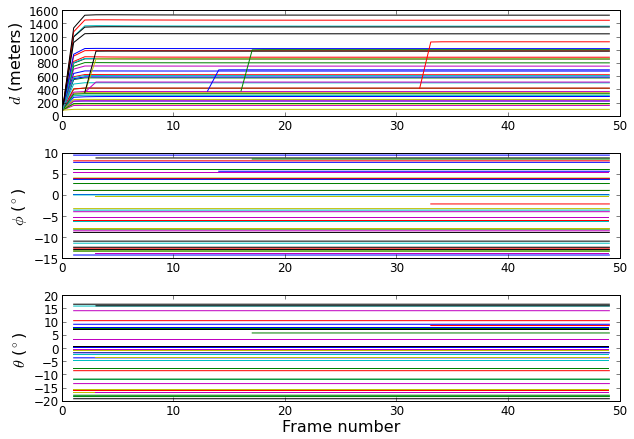
\includegraphics[scale=0.3]{./Figures/SimulationFigures/Figure6.png}
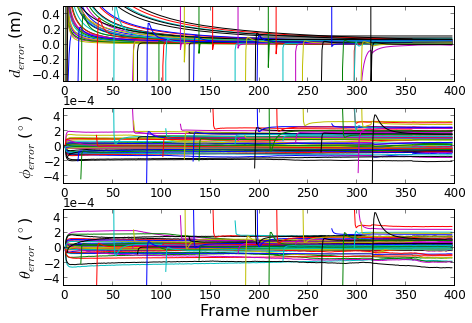
\includegraphics[scale=0.3]{./Figures/SimulationFigures/Figure7.png}
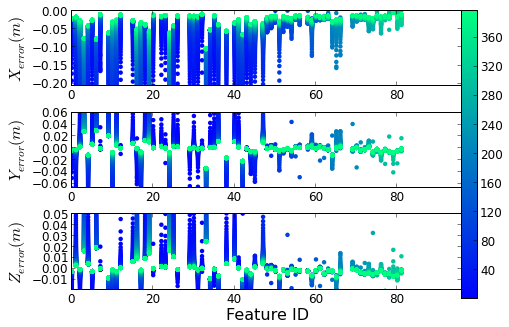
\includegraphics[scale=0.3]{./Figures/SimulationFigures/Figure5.png}
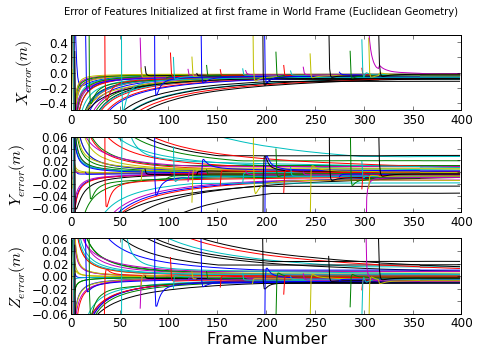
\includegraphics[scale=0.3]{./Figures/SimulationFigures/Figure8.png}
\caption{Features parameters and error convergence under no noise condition}
\label{fig:simfig5-8}
\end{figure}

\section{Effect of UAS Motion}

The simulation result from UAS forward travel shows that the 
CC\_EKF\_SLAM algorithm does feature tracking and self localization 
quite well under simple UAS motion. Next, the algorithm is tested with a 
more complex and realistic scenario. A series of motion is added to the 
simulation in addition to the forward motion. The remaining 5 types of 
maneuver are added one at a time. These maneuvers are: translation on Y, 
translation on Z, rotation on X, rotation on Y and rotation on Z. Each 
motion is modelled by a sine wave with frequency at 1Hz, and variable 
amplitude. For translation on Y and Z axis, the sine amplitude varies 
from 1 meter to 19 meters with 2 meters increments. For X, Y, and Z axis 
rotation, the amplitude varies from 0.001 radius to 0.018 radius with 
0.001 radius increment. 

\subsection{UAS Localization under Motion}

Figure \ref{fig:simfig9-10} shows the UAS localization error statistic 
under translation motion on Y and Z axis. Figure \ref{fig:simfig11-13}. 
shows the UAS localization error statistic under rotation motion on X, 
Y, and Z axis. The blue dots mark the mean value $\mu$ of the 
error throughout the tracking, and the error bars mark the standard 
deviation $\sigma$. 

The translation motion clearly increases the error of UAS localization. 
However, the amount of increase is insignificant. With the Sine 
amplitude increased to 19m, UAS position error increased by less than 
0.02 meter. 

On the other hand, rotation motions have a big impact on the accuracy of 
localization. Rotation on X axis has small effect on the accuracy of UAS 
position and orientation estimate. No obvious increase on mean and 
standard deviation of the error can be observed. Rotations on Y and Z 
axis yield significant error increase on the position of the UAS. 

\begin{itemize}
  \item Rotation on Y axis increases the UAS X position mean error, as
  well as the standard deviation. For Z positioning of the UAS, the
  mean error stays zero, but standard deviation increase dramatically.
  \item Same thing happens to the X and Y positioning for rotation on
  Z axis.
\end{itemize}

\begin{figure}[h]
  \centering
  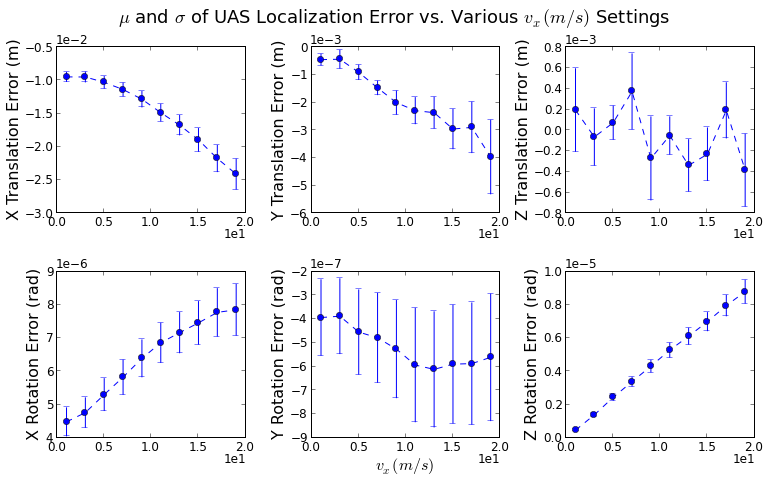
\includegraphics[scale=0.25]{./Figures/SimulationFigures/Figure9.png}
  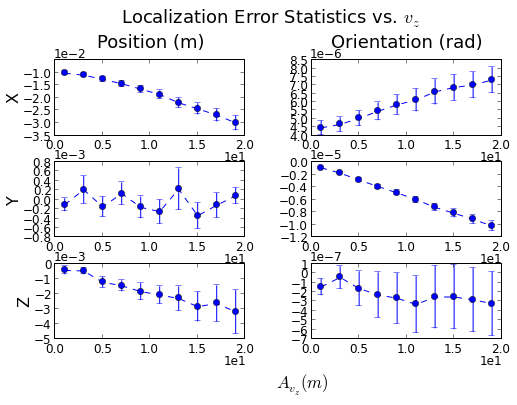
\includegraphics[scale=0.25]{./Figures/SimulationFigures/Figure10.png}
  \caption{UAS localization error under translational \label{fig:simfig9-10}
    motion}
  
\end{figure}

\begin{figure}[h]
  \centering
  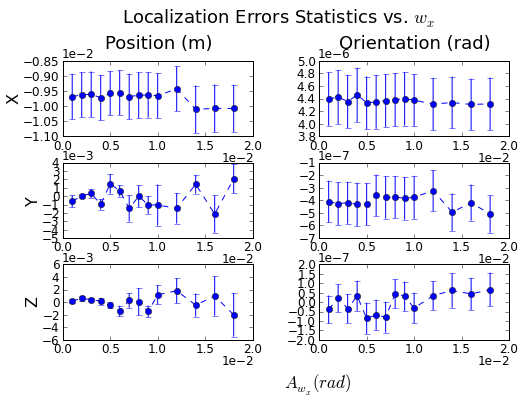
\includegraphics[scale=0.25]{./Figures/SimulationFigures/Figure11.png}
  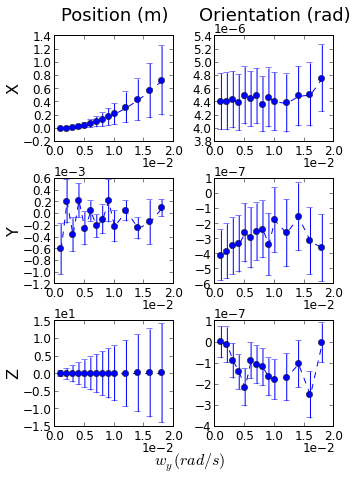
\includegraphics[scale=0.25]{./Figures/SimulationFigures/Figure12.png}
  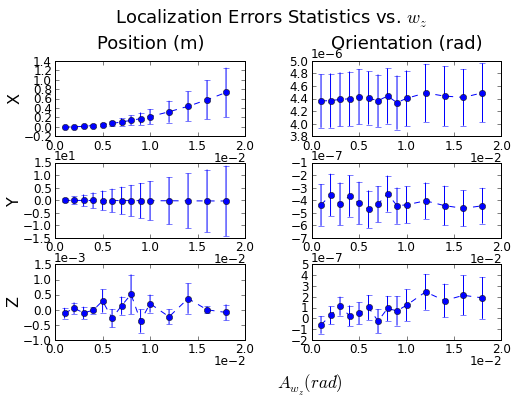
\includegraphics[scale=0.25]{./Figures/SimulationFigures/Figure13.png}
  \caption{UAS localization error under rotatioanl motion}
  \label{fig:simfig11-13}
\end{figure}

To understand how rotation motion affect the UAS localization
estimation, the UAS position on X, Y, Z in world frame are plotted
below (figure \ref{fig:simfig14}) with rotation amplitude on X, Y and
Z set at 0.01 radius. With rotation on X axis, the position error of
UAS shows some oscillation. The oscillation magnitude remains small
(in the scale of millimeters) and around zero. For rotation on Y and
Z, the situation is very different. Both rotation motions caused the
UAS position error to oscillate with the oscillation amplitude
increasing (diverging) as tracking goes on. The X position error of
the UAS increases in positive value with both rotation on Y and Z, but
the most significant impact happens on the Z position (for rotation on
Y) and Y position (for rotation on Z), with error reaching 20 meters
at the end of the video sequence. With rotation rate increases
(amplitude of the sine wave), the rate of error diverging from zero
also increases, hence, resulting in an increasing error standard
deviation in error statistic plots. This simulation result suggests
that CC\_EKF\_SLAM algorithm is very sensitive to rotation on Y and Z
axis.

\begin{figure}[h]
  \centering
  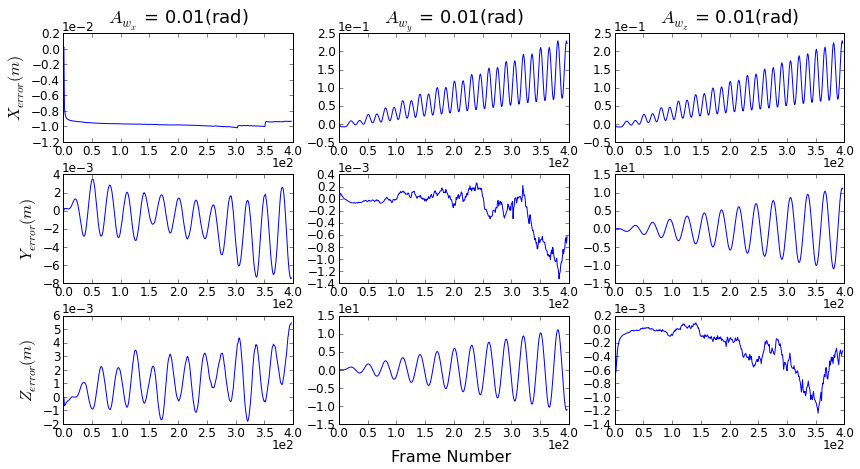
\includegraphics[width=14cm, keepaspectratio=true]{./Figures/SimulationFigures/Figure14.png}
  \caption{UAS estimated position in world frame}
  \label{fig:simfig14}
\end{figure}

\subsection{Feature Mapping Accuracy under Motion}

Feature mapping error statistic are drawn from the feature error at last 
frame, since features error converge to zero as tracking goes on. 
Figure \ref{fig:simfig20-21} shows the feature mapping error statistic 
with translation motion on Y and Z axis. Translation motions increase 
both the error mean and standard deviation, but not by much. With the 
motion maximum amplitude ranging from 1 meters to 19 meters, the 
increases of features position error mean and standard deviation are 
both in the scale of centimeters.

\begin{figure}[h]
  \centering
  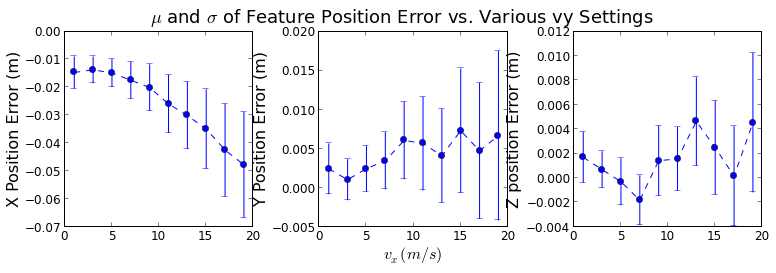
\includegraphics[scale=0.5]{./Figures/SimulationFigures/Figure20.png}
  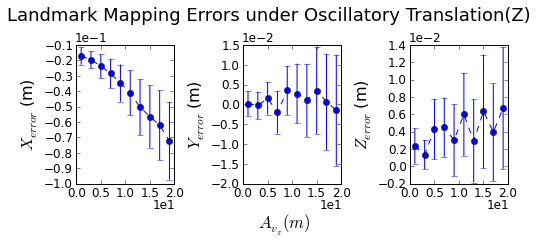
\includegraphics[scale=0.5]{./Figures/SimulationFigures/Figure21.png}
  \caption{Feature mapping error under rotatioanl motion}
  \label{fig:simfig20-21}
\end{figure}

Figure \ref{fig:simfig22-24}. shows the feature mapping error statistic 
for rotation motion on X, Y and Z axis. With maximum rate of rotation 
ranging from 0.001 rad/frame to 0.018 rad/frame

\begin{figure}[h]
  \centering
  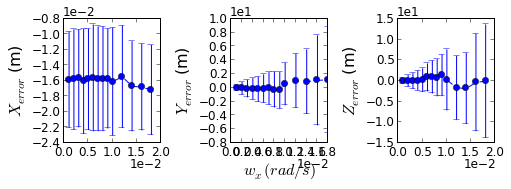
\includegraphics[scale=0.5]{./Figures/SimulationFigures/Figure22.png}
  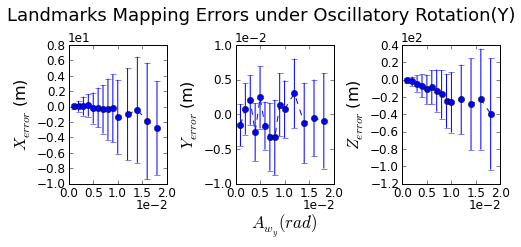
\includegraphics[scale=0.5]{./Figures/SimulationFigures/Figure23.png}
  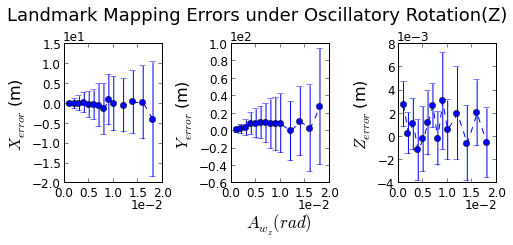
\includegraphics[scale=0.5]{./Figures/SimulationFigures/Figure24.png}
  \caption{Feature mapping error under rotatioanl motion}
  \label{fig:simfig22-24}
\end{figure}


\begin{itemize}
  \item Rotation on all three axis yields significant error increase
  for feature position estimation
  \item X axis rotation causes increase on standard deviation of Y and
  Z axis feature position error, and by similar amount. The error are
  in scale of meters with maximum rotation setting.
  \item Y axis rotation causes increase on mean and standard deviation
  of X and Z axis feature position error. Z axis feature position
  receives the biggest impact with error in the scale of hundreds of
  meters with maximum rotation setting
  \item Z axis rotation impacts on X and Y axis feature position in a
  similar way as the Y axis rotation.
\end{itemize}

\begin{figure}[h]
  \centering
  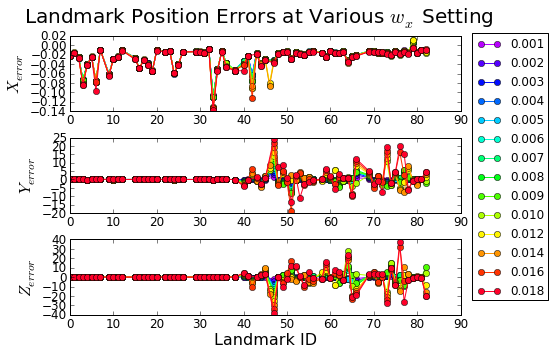
\includegraphics[scale=0.5]{./Figures/SimulationFigures/Figure17.png}
  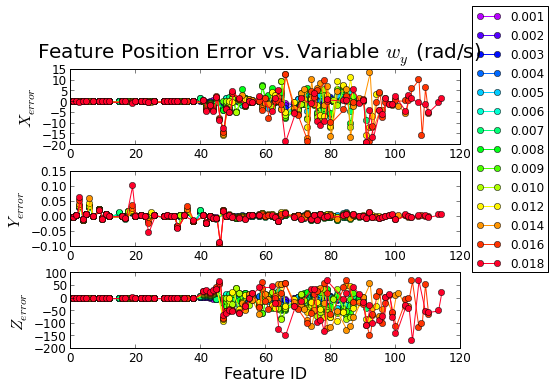
\includegraphics[scale=0.5]{./Figures/SimulationFigures/Figure18.png}
  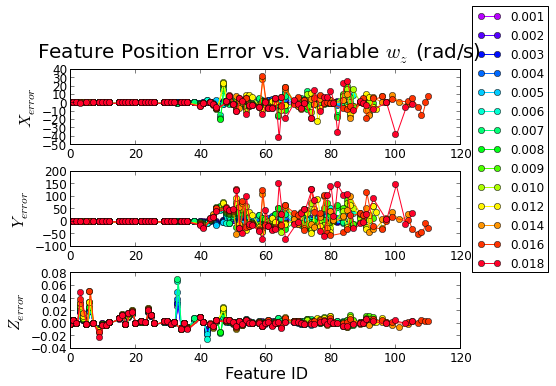
\includegraphics[scale=0.5]{./Figures/SimulationFigures/Figure19.png}
  \caption{Feature mapping error under rotatioanl motion}
  \label{fig:simfig17-19}
\end{figure}

Figure \ref{fig:simfig17-19} shows the features position error at the last
tracking frame for all three type of rotation motion. The errors are
plotted against feature ID and it revealed some more characteristic of
the features mapping errors.

\begin{itemize}
  \item With rotation on Y and Z, the tracked features easily went out
  of FOV. This can be observed from total number of features went from
  80 to over 110 with Y axis rotation setting varied from 0.001rad/s
  to 0.018rad/s. This caused frequent addition of new features.
  \item Features added after first frame has much bigger error than
  features added at first frame. At 1$^{st}$ frame, 40 features added
  to the filter. Error plots from Y and Z axis rotation both shows
  that major feature mapping error came from features added after the
  1 $^{st}$ frame with ID bigger than 40.
\end{itemize}

To investigate how does rotation motion results in bigger error on
features added after first frame, feature parameters error (converted
to world frame) with $wy = 0.01$ are plotted in
figure \ref{fig:simfig25}. It is found that the most significant
error happen to parameter $\phi$ which is the feature elevation angle.
This angle has the same definition as rotation angle around Y axis.
The second contributor is $z_i$ (the Z axis coordinate of the feature
initialization point). The both parameters have an offset error at
initialization, and were never corrected throughout the tracking.

Figure \ref{fig:simfig26} shows the $\phi$ error at 
initialization in camera frame and world frame. The blue line shows the 
error in camera frame. The red line shows the error in world frame 
transformed using the estimated UAS position and orientation. It is 
clear that it is the transformation process that introduced the offset 
error in $\phi$. Offset error in $z_i$ is due to the same 
reason. Recall that with Y axis rotation, UAS localization estimate has 
biggest error in X and Z axis coordinates estimate. Features initialized 
at first frame don't carry any offset error is because the 
transformation process is using the same parameters in both way. During 
tracking, these features are transformed to the new camera frame using 
the estimated UAS position and orientation. These are the same 
estimation being used to transform feature position from camera frame 
into world frame. Therefore, although the UAS localization estimations 
are different from the ground truth, feature initialized at first frame 
were not affected. To conclude, the major contributor for feature 
mapping error came from error in UAS localization estimation.

\begin{figure}[h]
  \centering
  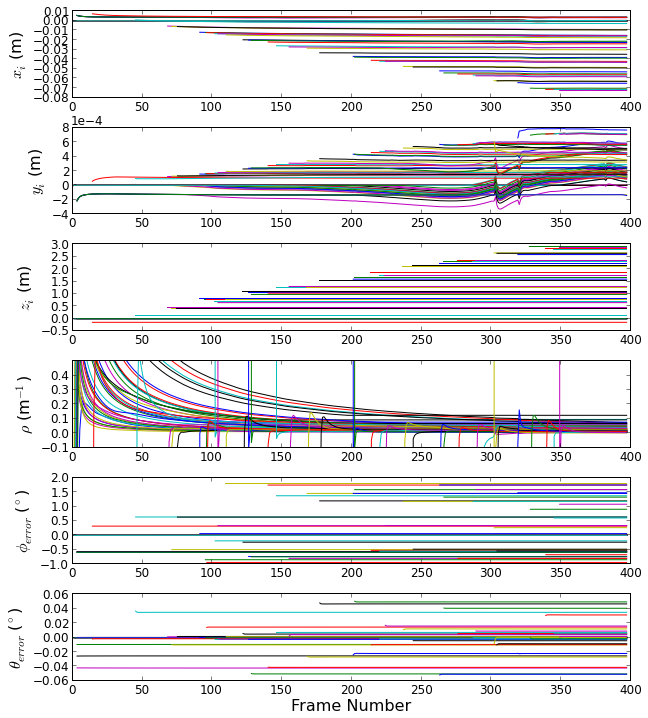
\includegraphics[scale=0.5]{./Figures/SimulationFigures/Figure25.png}
  \caption{Feature parameters error under rotatioanl motion}
  \label{fig:simfig25}
\end{figure}

\begin{figure}[h]
  \centering
  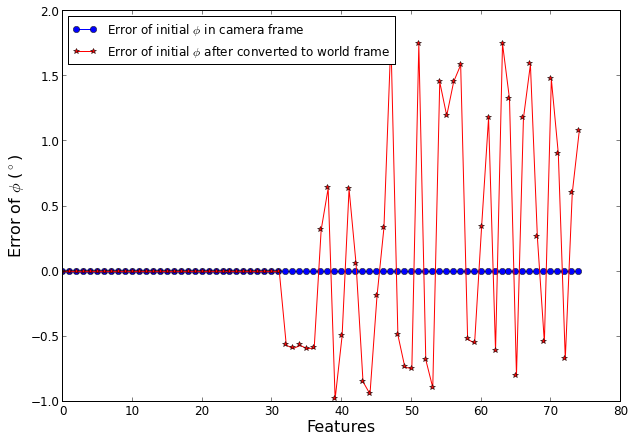
\includegraphics[scale=0.5]{./Figures/SimulationFigures/Figure26.png}
  \caption{Error of $\phi$ in camera frame and world frame at initialization}
  \label{fig:simfig26}
\end{figure}


\section{Camera Intrinsic Parameters}
This section summarizes the impact of inaccurate camera parameters 
estimations. Error on camera intrinsic parameters is simulated by using 
different values for camera models. One model is used in the simulator 
to project 3D points onto image plane, and the other is used in the 
measurement model of CC-LK-SLAM. $c_{x}$, $c_{y}$, $f_{x}$, and 
$f_{y}$ are simulated individually and distortion parameters $[k1, 
k2, p1, p2]$ are simulated as a group. Using the calibrated camera 
model (see section ???) as a base model,$ c_{x}$, $c_{y}$, $f_{x}
$, and $f_{y}$ in simulator camera model varied from -50\% to 50\% of 
the base model. Distortion parameters varied from 0\% to 140\% of the 
base model. 

\subsection{Effect from $(c_{x}, c_{y})$}

Figure \ref{fig:simfig34-35} show an over view of UAS localization
error statistics with incorrect estimates of $ (c_{x}, c_{y})$.

\begin{figure}[h]
  \centering
  \includegraphics[scale=0.5]{./Figures/SimulationFigures/Figure34.png}
  \includegraphics[scale=0.5]{./Figures/SimulationFigures/Figure35.png}
  \caption{UAS localization error statistic with varying $(c_x, c_y)$}
  \label{fig:simfig34-35}
\end{figure}

UAS position error is dependent on $(c_{x}, c_{y})$ and time (figure
\ref{fig:simfig36-37}). The UAS position error is diverging (increases
in time), and can be modeled by 1 $^{st}$ order polynomial function,
with the rate of diverging decided by the error of $(c_{x}, c_{y})$.
$c_{x}$ affects UAS position on X and Y axis, and $c_{y}$ affects UAS
position on X and Z axis.

\begin{figure}[h]
  \centering
  \includegraphics[width=7cm,keepaspectratio=true]{./Figures/SimulationFigures/Figure36.png}
  \includegraphics[width=7cm,keepaspectratio=true]{./Figures/SimulationFigures/Figure37.png}
  \caption{Diverging UAS position error}
  \label{fig:simfig36-37}
\end{figure}

The feature mapping error statistics from incorrect estimate of $
(c_{x}, c_{y})$ are plotted in figure \ref{fig:simfig28-29}. The
following characters can be observed from the plots:

\begin{itemize}
  \item Incorrect $c_{x}$ affect feature position on all axis, among
  which, X and Y axis see the most significant error.
  \begin{itemize}
    \item The further $c_{x}$ deviate from the true value, the further
    the features appear (positive X axis error).
    \item On Y axis, smaller $c_{x}$ make feature appear further to
    the optical axis than ground truth (positive error), and bigger
    $c_{x}$ make features appear closer (negative error).
    \item Incorrect $c_{x}$ also affect Z axis feature position, but
    by a much smaller amount.
  \end{itemize}
  \item Incorrect $c_{y}$ affect feature position on all axis
  similarly to $c_{x}$. Estimates on X and Z axis show most amount of
  error.
\end{itemize}

\begin{figure}[h]
  \centering
  \includegraphics[scale=0.5]{./Figures/SimulationFigures/Figure28.png}
  \includegraphics[scale=0.5]{./Figures/SimulationFigures/Figure29.png}
  \caption{Feature mapping error statistic with varying $(c_x, c_y)$}
  \label{fig:simfig28-29}
\end{figure}

Plotting feature position error as a function of features ground truth 
positions reveals more information on how incorrect $c_{x}$ and $
c_{y}$ affect feature mapping. Feature position error is a function of 
its ground truth position, and $c_{x}$ (or $c_{y}$). 

\begin{itemize}
  \item Error on X axis is proportional to the ground truth position
  on X. The further the feature is, greater the error. The degree of
  incorrectness in $c_{x}$ decide the slope of the error plot, greater
  the error in $c_{x}$, steeper the slope (figure
  \ref{fig:simfig32-33}, plot (a), subplot $[1,1]$).
  \item Feature position error on Y axis is also proportional to the
  ground truth position on X with the slope polarity dependent on the
  polarity of the error of $c_{x}$, and error plot slope dependent on
  the error of $c_{x}$.
  \item Feature position error on Z axis is proportional to the ground
  truth position on Z, with slope polarity dependent on the polarity
  of error of $c_{x}$, and slope dependent on the error of $c_{x}$.
\end{itemize}

$c_{y}$ affects feature position similarly to $c_{x}$ (figure
\ref{fig:simfig32-33}, plot (b)), except feature position error on Z
is dependent on ground truth position on X, and error on Y is
dependent on the ground truth position on Y.

\begin{figure}[h]
  \centering
  \includegraphics[scale=0.5]{./Figures/SimulationFigures/Figure32.png}
  \includegraphics[scale=0.5]{./Figures/SimulationFigures/Figure33.png}
  \caption{Feature mapping error vs. ground truth feature position}
  \label{fig:simfig32-33}
\end{figure}

\subsection{Effect from $(f_x, f_y)$}

With $(f_x, f_y)$ varying from -50\% to +50\% of the calibrated
value, the UAS localization error is shown in \ref{fig:simfig45-46}.
For all $f_x$ and $f_y$ settings, UAS position error remained less than
+/-0.05 meters, and orientation error remained in less than 8e-6
radius. Compared to the error obtained from the ideal case simulation,
Error in $(f_x, f_y)$ estimation does not introduce any additional error into
UAS localization estimate. 
\begin{figure}[h]
  \centering
  \includegraphics[width=7cm,keepaspectratio=true]{./Figures/SimulationFigures/Figure45.png}
  \includegraphics[width=7cm,keepaspectratio=true]{./Figures/SimulationFigures/Figure46.png}
  \caption{UAS localization error statistic with variable $(f_x, f_y)$}
  \label{fig:simfig45-46}
\end{figure}

Feature mapping, on the other hand, is unavoidly affected by the error
in $(f_x, f_y)$ since these are the scaling factor that project
features from 3D world onto image plane. Figure \ref{fig:simfig38-39}
shows the error statistic of feature position estimation under
variation of $(f_x, f_y)$. The effect on the X axis component is
minimum, in the scale of milli meter. Y axis component receive the
most impact with unmatched $f_x$, since this is the scale factor that
map feature's Y component in world frame onto U axis on image plane by
$u = Y/X*f_x$. Same goes for the Z axis component of the feature
position estimate and its relation to $f_y$.
\begin{figure}[h]
  \centering
  \includegraphics[width=10cm,keepaspectratio=true]{./Figures/SimulationFigures/Figure38.png}
  \includegraphics[width=10cm,keepaspectratio=true]{./Figures/SimulationFigures/Figure39.png}
  \caption{Feature mapping error statistic with variable $(f_x, f_y)$}
  \label{fig:simfig38-39}
\end{figure}

Plotting the feature mapping error against feature ground truth
position reveals how error in $(f_x, f_y)$ estimate impact on feature
position estimate. When $f_x$ estimate contains error, Y component of
feature position is determined by the feature's ground truth position
on X and Y components. The value of $Y_{error}$ is directly portional
to the Y component of its ground trurth position, with the error in
$f_x$ determines the function's slope. Same relation can be found for
$Z_{error}$ with $f_y$, and $Z_{ground truth}$.

% TODO simfig38-39:Merge these two into one, showing only the related.
\begin{figure}[h]
  \centering
  \includegraphics[width=10cm,keepaspectratio=true]{./Figures/SimulationFigures/Figure42.png}
  \includegraphics[width=10cm,keepaspectratio=true]{./Figures/SimulationFigures/Figure43.png}
  \caption{Feature mapping error plotted against feature ground truth
    for various $(f_x, f_y)$}
  \label{fig:simfig38-39}
\end{figure}

\subsection{Effect from Distortion}

%%% Local Variables:
%%% mode: latex
%%% TeX-master: "thesis"
%%% End:

\end{document}

%%% Local Variables: 
%%% mode: latex
%%% TeX-master: t
%%% End: 
